%%%%%%%%%%%%%%%%%%%%%%%%%%%%%%%%%%%%%%%%%
% Masters/Doctoral Thesis 
% LaTeX Template
% Version 2.5 (27/8/17)
%
% This template was downloaded from:
% http://www.LaTeXTemplates.com
%
% Version 2.x major modifications by:
% Vel (vel@latextemplates.com)
%
% This template is based on a template by:
% Steve Gunn (http://users.ecs.soton.ac.uk/srg/softwaretools/document/templates/)
% Sunil Patel (http://www.sunilpatel.co.uk/thesis-template/)
%
% Template license:
% CC BY-NC-SA 3.0 (http://creativecommons.org/licenses/by-nc-sa/3.0/)
%
%%%%%%%%%%%%%%%%%%%%%%%%%%%%%%%%%%%%%%%%%

%----------------------------------------------------------------------------------------
%	PACKAGES AND OTHER DOCUMENT CONFIGURATIONS
%----------------------------------------------------------------------------------------

\documentclass[
11pt, % The default document font size, options: 10pt, 11pt, 12pt
%oneside, % Two side (alternating margins) for binding by default, uncomment to switch to one side
english, % ngerman for German
singlespacing, % Single line spacing, alternatives: onehalfspacing or doublespacing
%draft, % Uncomment to enable draft mode (no pictures, no links, overfull hboxes indicated)
%nolistspacing, % If the document is onehalfspacing or doublespacing, uncomment this to set spacing in lists to single
%liststotoc, % Uncomment to add the list of figures/tables/etc to the table of contents
%toctotoc, % Uncomment to add the main table of contents to the table of contents
%parskip, % Uncomment to add space between paragraphs
%nohyperref, % Uncomment to not load the hyperref package
headsepline, % Uncomment to get a line under the header
%chapterinoneline, % Uncomment to place the chapter title next to the number on one line
%consistentlayout, % Uncomment to change the layout of the declaration, abstract and acknowledgements pages to match the default layout
]{MastersDoctoralThesis} % The class file specifying the document structure
\usepackage[noend]{algpseudocode}
\usepackage{algorithmicx,algorithm}
\usepackage{subfig} %subfloat
\usepackage[utf8]{inputenc} % Required for inputting international characters
\usepackage[T1]{fontenc} % Output font encoding for international characters
\usepackage[UTF8]{ctex} % support for chinese
\usepackage{mathpazo} % Use the Palatino font by default
\usepackage{amsmath}
\usepackage{cite}
%\usepackage[backend=bibtex,style=authoryear,sorting=ynt]{biblatex} % Use the bibtex backend with the authoryear citation style (which resembles APA)
\usepackage{csvsimple}
%\addbibresource{ref.bib} % The filename of the bibliography
\usepackage{pdfpages}
\usepackage[autostyle=true]{csquotes} % Required to generate language-dependent quotes in the bibliography
\usepackage{indentfirst} 
\setlength{\parindent}{2em}
% \noindent
%----------------------------------------------------------------------------------------
%	MARGIN SETTINGS
%----------------------------------------------------------------------------------------

\geometry{
	paper=a4paper, % Change to letterpaper for US letter
	inner=2.5cm, % Inner margin
	outer=3.8cm, % Outer margin
	bindingoffset=.5cm, % Binding offset
	top=1.5cm, % Top margin
	bottom=1.5cm, % Bottom margin
	%showframe, % Uncomment to show how the type block is set on the page
}

%----------------------------------------------------------------------------------------
%	THESIS INFORMATION
%----------------------------------------------------------------------------------------

\thesistitle{} % Your thesis title, this is used in the title and abstract, print it elsewhere with \ttitle
%\supervisor{} % Your supervisor's name, this is used in the title page, print it elsewhere with \supname
\degree{} % Your degree name, this is used in the title page and abstract, print it elsewhere with \degreename
\author{
 } % Your name, this is used in the title page and abstract, print it elsewhere with \authorname


\keywords{} % Keywords for your thesis, this is not currently used anywhere in the template, print it elsewhere with \keywordnames
\university{} % Your university's name and URL, this is used in the title page and abstract, print it elsewhere with \univname
\department{} % Your department's name and URL, this is used in the title page and abstract, print it elsewhere with \deptname
\group{} % Your research group's name and URL, this is used in the title page, print it elsewhere with \groupname
\faculty{} % Your faculty's name and URL, this is used in the title page and abstract, print it elsewhere with \facname


\begin{document}

\frontmatter % Use roman page numbering style (i, ii, iii, iv...) for the pre-content pages

\pagestyle{plain} % Default to the plain heading style until the thesis style is called for the body content

%----------------------------------------------------------------------------------------
%	TITLE PAGE
%----------------------------------------------------------------------------------------

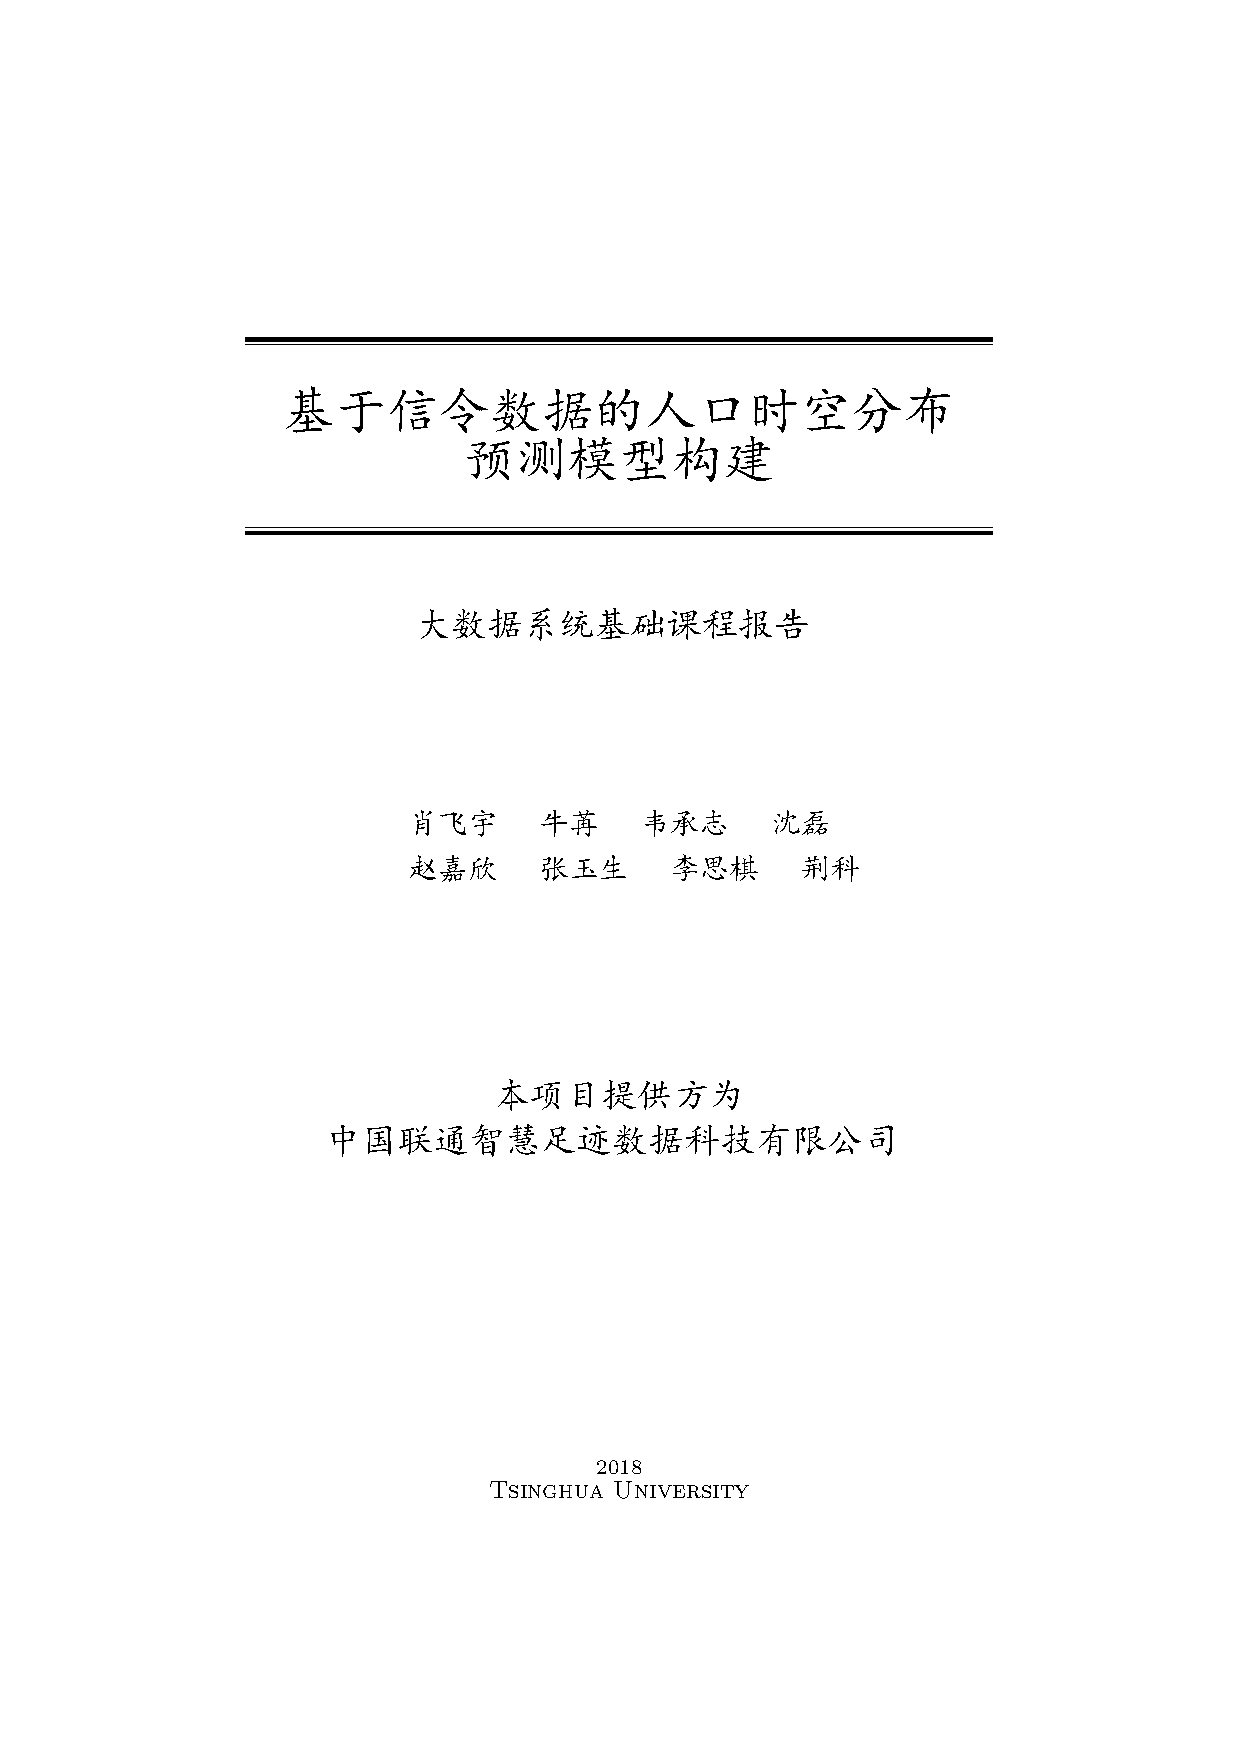
\includepdf[pages=-]{cover.pdf}
%----------------------------------------------------------------------------------------
%	DECLARATION PAGE
%----------------------------------------------------------------------------------------


\cleardoublepage

%----------------------------------------------------------------------------------------
%	QUOTATION PAGE
%----------------------------------------------------------------------------------------

\vspace*{0.2\textheight}

\noindent\enquote{\itshape What magical trick makes us intelligent? The trick is that there is no trick. The power of intelligence stems from our vast diversity, not from any single, perfect principle.}\bigbreak

\hfill Marvin Minsky

\vspace*{0.05\textheight}

\noindent\enquote{\itshape All models are wrong, but some are useul.}\bigbreak

\hfill G.E.P. Box

%----------------------------------------------------------------------------------------
%	ABSTRACT PAGE
%----------------------------------------------------------------------------------------

\begin{abstract}
\addchaptertocentry{\abstractname} % Add the abstract to the table of contents
对于城市特别是大型城市而言,预测人口的流动和分布变化对于城市交通治理、公共安全和危险评估都有着重要的战略意义。 而由于其受到诸如区域间交通、突发事件、天气等复杂因素的多元影响,利用传统方法对于其进行预测十分困难。\\
\\
我们将城市分割成均匀网格,基于交通、气象、时间和事件等多源信息,
设计了期望输出为驻留人数、出发人数、到达人数有监督人工神经网络,综合预测未来每个网格的进入和流出人流数。 网络的输入为数据的特征,通过对于数据的预处理和分析我们认为主要和人数与星期、具体小时、位置、天气、前一小时的人数等主要因素有关。同时我们以获得数据中的驻留人数、出发人数、到达人数作为标签,利用期望输出与网络输出之间的误差建立学习信号反向传播,修正网络权重,最终得到了相对较理想的预测结果。
\end{abstract}

%----------------------------------------------------------------------------------------
%	ACKNOWLEDGEMENTS
%----------------------------------------------------------------------------------------

\begin{acknowledgements}
\addchaptertocentry{\acknowledgementname} % Add the acknowledgements to the table of contents
感谢中国联通智慧足迹数据科技有限公司提供的数据支持和相关指导,感谢大数据系统课程的各位老师和助教的帮助。
\end{acknowledgements}

%----------------------------------------------------------------------------------------
%	LIST OF CONTENTS/FIGURES/TABLES PAGES
%----------------------------------------------------------------------------------------

\tableofcontents % Prints the main table of contents

\listoffigures % Prints the list of figures

\listoftables % Prints the list of tables


%----------------------------------------------------------------------------------------

\mainmatter % Begin numeric (1,2,3...) page numbering

\pagestyle{thesis} % Return the page headers back to the "thesis" style

% Include the chapters of the thesis as separate files from the Chapters folder
% Uncomment the lines as you write the chapters

% Chapter 1

\chapter{引言} % Main chapter title
\label{Chapter1} % For referencing the chapter elsewhere, use \ref{Chapter1} 
\section{背景介绍:从预测人口流动的城市危机防范到城市计算}
进入新千年以来,迅速发展的城市化进程催生了很多超大和大城市,并深远地改变了城市居民的生活状态和方式,然而,这也催生了诸如城市空气恶化、交通堵塞等重大挑战。而在这其中,对于城市人口流动的管控和风险预测也显得十分重要。
预测城市人口的流动对于现代城市的安全和管理都是一个十分重要而充满挑战性的问题,而随着城市体量和现代交通、信息等的发展,这一问题显得尤为重要。 2014年的新年夜,由于人流的急剧变化和缺乏应急预警,在上海外滩发生了造成36人死亡、47人受伤的惨痛踩踏事故\cite{hoang2016fccf:}。 试想,如果当时能有可以预测人流变化和区域流动的方法,对于这一区域进行及时的预警和疏导,就不会有这样的惨剧发生。\\
关于人流预测的先前研究集中于对于单个个体的活动的预测分析\cite{ye2009mining,zheng2012an}和对道路的交通状况的研究\cite{shang2014inferring,wang2014travel}。 尽管这些研究从一定程度上提供了对于城市的交通、人流的详细描述,但是由于整个城市的规模之大,要想对于整个城市或者城市的一部分进行这样的模拟来预测人口的流动在模拟能力和花费上是难以接受的;同时,对于整个城市的个体进行如此细致的模拟对于预测人口流动又显得没有必要。 另外,仅仅研究个体的行为无法揭示从群体层面上所会“涌现”出的诸多特征。\\
和传统的方法不同,由于现代的感知技术和大规模计算能力的成熟使得获取和计算和分析城市的巨量数据成为了可能,这也就催生出一个新的技术领域和框架——城市计算。这里本文将首先给出对于“城市计算”的基本介绍和核心要点以及其在预测城市人口流动这一问题中的结合和应用。\\
城市计算是一个获取、整合和分析城市空间中各种来源 (如传感器、设备、车辆、建筑物和人类) 生成的大型异构数据的过程,用以解决城市面临的主要问题\cite{zheng2014urban}。 城市计算连接无处不在的传感技术、先进的数据管理和分析模型以及新颖的可视化方法, 以改善城市环境、人类生活质量和城市运营体系。
\section{城市计算}
\subsection{框架}
如图\ref{fig:1.1}所示,城市计算主要由城市感知和数据获取、城市数据管理、城市数据分析和服务提供等环节构成。
\begin{figure}[ht]
\centering
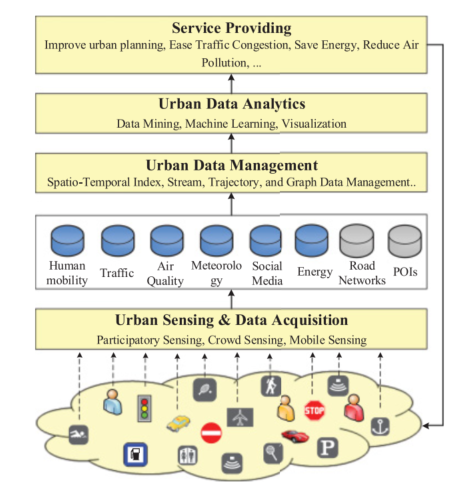
\includegraphics[width=0.8\textwidth]{frame.png}
\caption{城市计算的基本框架\cite{zheng2014urban}}
\label{fig:1.1}
\end{figure}
在城市感知阶段,主要利用固定的传感器和移动的如GPS信号、手机信号甚至社交媒体内容等多方面多维度的数据来源进行城市信息的收集;在城市数据管理阶段,将获得的不同来源甚至不同组织形式的数据进行结构化管理并进行和时间和空间上的对应以备后续分析;在数据分析环节,首先对于得到的组织数据进行模式分析,同时对于异常情况的发生可以进行准确的识别和预测;最后在服务提供阶段,对于异常的预测可以及时地对于相应的群体进行信息的分发还可以提供给城市的管理者进行及时的预警和调控。
\subsection{主要挑战}
和其他相对简单的系统相比,城市系统有着相对复杂的层级结构和纷繁的相互交织影响的动态信息,其作为一个动态复杂系统必然展现出诸如“涌现”等信息交织变化的特征\cite{anderson1972more},从而对于其的分析和预测必然面临着在不同层次和角度上的挑战。而城市计算主要有下面三个主要的挑战:
\subsubsection*{城市感知和数据获取}
在城市的大尺度下,想要连续地获得全面的数据显得十分困难。 例如,追踪某个区块的道路的车流相对可以实现,但是要连续追踪整个城市的车流由于传感器的分布和数据的传输等原因显得难以实现。 值得注意的是,相比传统的技术手段,在城市计算的框架下,人类所提供的信息或许可以成为这种传统的数据获取缺失的一种补充。 例如, 人在社交媒体上公开发表内容可能会提供周边环境的一些诸如交通、天气等的一些信息。 考虑到现代通讯的发达和城市人口的体量,这一信息来源蕴含着巨大的可以挖掘的信息,然而,这一新的数据来源再提供新的数据可能的同时也造成了新的问题:
\begin{itemize}
	\item 关于个人信息收集和隐私保护的问题
	\item 信息的难以控制和不均匀分布性。 传送信息的人的时间、地点、信息的内容、形式等式难以控制的,而且并不是能连续获得的,这也就造成了数据缺失和信息稀疏的问题,同时在城市中,无论从空间和时间上,从人类活动得到的信息都不是均匀分布的,这也对数据的分析造成了困难
	\item 由人所产生的数据可能是非结构化、不明显甚至充满噪声的,这和传统的传感器的信息可以直接用于清晰的解释和分析十分不同
\end{itemize}

\subsubsection*{异构数据的分析}
首先,城市计算所面临的数据往往是异构数据,也就是说对其进行分析和研究需要考虑一系列的复杂因素。 比如,对于空气质量的研究需要连续考量交通流、城市气象变化乃至土地区块利用情况等多重综合因素。 而现有的无论是数据挖掘还是机器学习等技术都只针对一种数据进行研究。 当然,一种显然的想法是将从不同的数据源提取的数据进行相同处理 (例如, 简单地
将这些特征放入要素向量并将其放入分类模型中),然而这种做法已经被证明预测的准确性相对较差\cite{yuan2012discovering}。 所以,如果采用多重的数据集进行分析会使得数据的维度增加,而这又加重了本就存在的数据集的稀疏问题, 如果这一问题没有被妥善处理,这甚至反而会造成模型的准确度下降。 \\
其次,城市计算的很多场景需要及时的预测和反馈,如空气污染、人流预测。这就要求分析手段既要保证分析的准确性还要保证其处理花费的有限性。
\\
最后,城市尺度的多维数据规模对于数据的可视化也提出了挑战,而数据分析结果的可视化能否提供足够清晰的信息也关系到其分析结果能否在灾害避免、交通疏导、空气治理等决策过程中发挥作用。
\subsubsection*{虚拟世界和现实世界的交互}
和传统的编写一个大型游戏或者是构建一个搜索引擎几乎完全在虚拟世界进行构建不同,城市计算从数据的获取、分析到最后的预测都不可避免的和城市的现实运行产生联系,这就给这样的系统的设计提出了新的信息交互和处理的挑战。
\subsection{城市信息}
之前提到,城市内部有着纷繁众多的信息来源,诸如地理信息、交通信息、手机信号、社交网络信息甚至经济运行的信息等多方面的信息。 在这一部分,本文将针对进行人流预测分析所主要依托的几个信息来源进行介绍和阐述
\subsubsection*{地理信息}
地理信息主要包括路网信息和地理坐标信息,可以预料到,对于城市的诸多活动,路网都是一个很关键的因素,而位于其中的一些居住区、商场、餐厅的地理信息也对于分析十分重要。
\subsubsection*{交通信息}
交通的智能化和网联化,如打车服务软件的广泛使用使得对于一部分(出租车等)交通信息的实时收集变得可能,而城市道路上分布广泛的摄像头和传感器也提供了长期而巨量的交通监测信息。值得注意的是,广泛搭载GPS的车辆的运行可以提供连续的时空和轨迹信息。
\subsubsection*{移动手机}
由于移动手机实时和基站交换信息,通过这可以得到手机持有者的当前位置,再通过不同基站的信号可以获知其轨迹移动。由于智能手机的广泛使用,这一信息实际上提供了对于人流预测十分关键的基础信息。
\subsection{城市计算的技术手段}
为了应对之前所提到的三点挑战,研究者提出了很多技术和手段,其可以被大致分为以下四个方面:
\begin{itemize}
	\item 城市感知和数据处理技术
	\item 异构数据的融合技术
	\item 稀疏数据的处理方法
	\item 数据可视化的手段
\end{itemize}
\subsubsection*{城市感知和数据处理}
对于城市的数据获取,首先是依赖传统的传感器等手段进行数据的获取,其次可以通过对人群产生的数据进行处理得到所需求的数据,如可以通过网络信息的处理得到一些特定区块的餐饮经营状况。 \\
而对于数据的处理首先需要注意的是城市数据往往伴随着时间和空间信息,而处理机制需要能对于这样的复杂信息进行快速而有效的处理。现有研究中通常有三种结构来进行处理:流数据、轨迹数据和图数据。 在本文后面的人流预测的工作中将采取图数据的形式进行分析,这里一并对于其他两种处理形式进行简要介绍。
\subsubsection*{流数据和轨迹数据}
流数据在生活中十分常见,如温度数据、电的使用量和传感器的视频记录,都是时序的流数据,而对于流数据的研究和处理早已有了相对成熟的体系和方法\cite{Aggarwal2006Data},一系列成熟的DSMSs(Data stream management sysytems)系统(如 StreamInsight)等已经得到广泛应用。\\
而轨迹数据是指移动物体在地理空间移动形成的点的坐标连线,而诸如携带 GPS 的车辆和移动手机的信号都能生成轨迹数据。 而相比流数据而言,轨迹数据由于其和地理位置的高度相关和时序上的先后关联,传统的流数据的处理方法遇到了相当大的困难\cite{Wang2011Computing}。
\subsubsection*{图数据}
与流数据和轨迹数据不同,图数据是一种很好的表示交通系统,社交网络,人流分布的数据结构形式。 之前的研究主要集中对于静态的图数据的处理\cite{angles2008survey},而在城市计算中,往往是有一系列有着时序特征的图数据,也称为时空图\cite{hong2015detecting}(Spatiotemporal graph, ST graph),
对于时空图数据的研究还在持续进行中。

\subsection{异构数据的融合技术}
在进行城市计算的过程中,需要利用很多的数据来源收集数据,这就必然要求要对不同来源和形式的数据进行统一化的处理从而进行下一步的分析。
现有的处理手段主要有以下三种:
\begin{enumerate}
	\item 在功能级别使用不同的数据源,即处理不同的数据源,同等地将从不同数据源提取的要素组合到一个特征向量。 需要注意的是,在分析前需要采用一定的方法对于数据进行归一化。这种方法也是目前采用最多的方法。
	\item 在不同的数据分析阶段采用不同的数据。 在文献中\cite{zheng2011urban}有将城市用路网划分为不同的区域再使用人的流动数据进行交通情况的预测分析。
	\item 将不同的数据输入到模型的不同部分。这一方法需要对于数据本身的深层理解才能构建出相对合理的模型,在实际的研究\cite{Zheng2013U,yuan2012discovering}中也发现基于对于数据的理解所构建的模型要显著好于前两种。
\end{enumerate}

\subsection{稀疏数据的处理方法}
尽管城市计算的数据规模非常之大,但是由于测量数据和测量手段的特点,依然会有数据缺失的问题,这就是是在计算机科学中经常需要处理的数据稀疏性的问题。 关于数据稀疏性的处理手段,常用和相对有效的有下面四种,在后文的工作中也会采取其中的方法对人口的信令数据进行预处理。
\subsubsection*{协作筛选}
协作筛选(Collaborative filtering, CF)被广泛使用在推荐系统的构建中,其基本的思想是相似的使用者对相似的物品有相似的评估标准和机制\cite{goldberg1992using}。 那么,如果可以确定出使用者和物品之间的联系,就可以对未来的使用者的评估做出预测\cite{nakamura1998collaborative}。 而在城市计算中, 物品可以是地理信息,乘客,司机还有服务的订购者。 一旦我们组装了矩阵,就可以使用这一准则来填充缺失的值。
\subsubsection*{矩阵分解}
矩阵分解,顾名思义就是讲矩阵分解为两个或者三个矩阵的乘积。 典型的方法有矩阵的 LU 分解、 QR 分解、 SVD 分解,其中 SVD 分解是使用最频繁的方法。 一种常用的方法为当矩阵非常稀疏时,可以使用三个低阶的矩阵对于其进行近似,比如只选取对应的奇异值之和大于总的奇异值之和的 \% 90 的那些行的数据。
\subsubsection*{张量分解}
张量通常有三个维度, 可以根据数据值对的特征分解为矩阵或向量的乘法。 限制分解的目标函数是最大限度地减少
中现有项的值的乘积。分解后, 我们通过
将分解后的矩阵或向量相乘可以填充张量中的缺失值。常常使用的主要有 PARAFAC\cite{bro1997parafac} 和 Tucker 分解\cite{kolda2009tensor}两种方法, 前者将张量分解为
三个向量的一系列乘积的总和, 而后者
用三个矩阵和一个核心张量的乘法近似一个张量。
\subsubsection*{半监督学习
}
半监督学习是一类监督学习任务和技术, 利用未标记的数据训练模型,其中通常包含少量标记的数据和大量未标记的数据。许多机器学习的研究人员发现, 未标记的数据, 当结合少量的标记数据,可以在学习精度方面有相当大的提高。 现有很多半监督的学习方法,如生成模型、基于图形的方法和协同训练。 具体来说,协同训练它假定每个实例都由两个
不同的功能集组成,这些功能集为每个实例提供了不同的和互补的信息。理想情况下, 每个实例的两个功能集都是有条件地独立,并且可以从每个视图准确地预测实例的分类。协同训练可以产生更好的推理结果, 因为其中一个分类器正确地标记了其他分类器以前错误分类的数据\cite{nigam2000analyzing}。\\

\subsection{数据可视化}
可视化以直观的方式帮助我们理解获取的知
识和模式。与单一数据可视化不同,城市计算中
的可视化技术需要同时考虑多个维度,其中,空间和时间是两个至关重要的维度\cite{zhengyu2015}。
% Chapter 2

\chapter{项目需求分析} % Main chapter title

\label{Chapter2} 
\section{用户背景介绍}
智慧足迹数据科技有限公司是中国联通集团控股,由中国联通和西班牙电信合资成立的专业大数据公司,依托中国联通卓越的数据能力、全球最强大的手机信令处理平台Smart Steps等产品技术和丰富的市场经验,提供位置信息洞察及相关大数据业务。\\
\indent 公司坚持对接国家战略,践行社会责任,落实集团关于大数据布局的战略思想,以“开垦、开放、开源”为发展战略,树立了“简单,成事”的企业文化,广泛集聚百度、高德、微软、Oracle、Teradata、HP、IBM、科研院所等国内外一流人才,打造了一支激情创业、价值导向、高效运营的大数据精英团队。\\
\indent Smart Steps是全球领先的位置大数据技术,利用匿名、聚合、外推的网络数据,经过高度自动化和深度降噪处理,将运营商数据加工成反映用户空间行为的时空标签,快速高效提供高价值的“线下位置+线上行为”的数据洞察服务。\\
\indent 公司通过“T”型产品战略赋能产业生态,横向开放合作,结合外部智脑综合利用数据,实现数据增值;纵向垂直应用,为行业客户提供全方位服务。公司以中国联通4亿+用户数据为基础,整合运营商、互联网、政府及商业等数据,采用AI化、标签化、模型化数据处理技术,自主研发10大产品平台,包含数据产品(统计数据集、统计数据API、能力开放DaaS平台、Data lab)、行业垂直产品(数据报告、实时热力及产业经济平台、数据可视化平台、极目洞察选址SaaS平台、金融风控平台、数字营销平台)等。\\
\indent 智慧足迹公司业务主要涵盖两个方面,分为产品平台和行业方案,这两者呈现相辅相成的关系,基于强大的信令数据资源和数据处理能力构建多元化的大数据平台,为不同需求的客户根据其不同的需求从不同的角度分析数据得出个性化的分析结果,从而得到不同行业解决方案。\\
\indent 数据平台分为数据智能平台,数据洞察平台,能力开放平台,数据引擎平台。其中数据智能平台中的统计数据集是基于联通用户的行为轨迹以及属性标签,通过SS平台的脱敏加工后,结合客户需求,实现不同时空、用户属性视角下的数据统计。产品以Excel或者CSV表格的形式对外提供(可选制图与报告配套销售),内容为统计数据集,客户可基于数据结果直接进行问题的研究以及分析决策。产品的主要功能是职住娱的分布、通勤和游憩、全目的的出行、人口动态变化、跨省跨域迁徙等。统计数据API将城市以250M边长的网格均匀覆盖,以接口调用形式访问,提供每一网格(或区域)各维度的人群特征属性,为进一步开展商业洞察、选址分析、指数评估、潜客挖掘提供数据依据。产品功能主要有基础人流数据、人群画像数据、人群流动数据、人群社会属性数据等。\\
\indent 极目洞察选址SaaS平台归属于数据洞察平台,通过简洁友好的交互界面,帮助客户快速监测定点区域周边客群资源,包括:客群规模、驻留特征、客群结构、消费能力、手机终端品牌、互联网偏好特征等;并基于行业模型为增量布点选址提供大数据决策支持。主要功能有,批量点洞察,自定义区域洞察,特定客群分布,自动推荐点位,定位评估等。实时热力及产业经济平台基于手机信令的实时热力产品是通过对手机信令进行实时处理和计算、分析,得出指定区域的实时人口特征,包括区域人口热力分布、人口数量、人口结构、人口来源、人口画像、人口迁徙、职住等信息。提供的产品形态包括:API数据接口或web页面。可为政府人口统计、应急监控及实时客流分析提供有价值的决策依据。主要功能有区域人口统计,人口流动统计,人口实时热力,区域人口结构,区域人口画像,人口职住分析等。数字营销平台依托中国联通的海量数据以及位置标签能力,在确保数据隐私安全的前提下,通过大数据的深入挖掘和分析为各行业客户优化投放策略和渠道,提供精准的营销触达手段。主要功能有标签定制,标签筛选,内容定制,营销策略定制,渠道灵活选择,营销监控,盘点及评估。金融风控平台在充分保障用户隐私安全的前提下,金融风控平台利用联通数据资源优势和领先的数据建模能力,提供反欺诈、信息核验和风险评估服务。帮助合作伙伴解决事前预防、事中防控、事后失联客户复联等业务流程相关的风险控制问题,达到降低业务风险,避免损失的效果。产品功能包括,职住验证,实时位置比对等。\\
\indent 数据能力开放DaaS平台,基于海量的联通多维数据,采用Hadoop大数据生态体系搭建集群,支持Spark、Hive等多种大数据挖掘及建模技术的应用。为客户提供基于位置的洞察、选址、营销等数据分析服务。平台用户可以通过接口的形式,运行各类定制化数据模型,安全合规的获取维度丰富的统计数据集结果,以满足行业应用的需求。产品功能主要有,区域洞察,客群发现,自主建模,主要可用于商业地产洞察,零售店选址,户外媒体点位洞察等。大数据可视化平台是公司自主研发的大数据产品,采集中国联通全国用户的手机信令数据和CRM系统属性数据,通过数据清洗、加工、处理和挖掘,运用领先的可视化技术,直观呈现海量数据隐含的巨大价值,提供人口监测与疏解、交通规划、公共安全、市场洞察等多样化决策支持。主要功能有人口分布,出行分析,跨域迁徙路线,区域人口洞察,选址分析,人流预警,可用于城市规划+智慧城市,职住分布+OD分析。\\
\indent 此外在数据引擎平台,还提供位置标签,即经SmartSteps信令处理平台加工,表达用户特征并满足客户需求的的集合数据。 AI业务模型:基于多源数据,利用机器学习等大数据技术和算法,构建行业场景应用模型。以及AI业务模型,基于多源数据,利用机器学习等大数据技术和算法,构建行业场景应用模型。\\
\indent 行业方案主要提供一下四个方面的服务,城市规划,政府治理,商企洞察,金融风控。城市规划设计人口分布分析,城市出行分析,城市间跨域迁徙分析,城市产业经济分析等。公司目前已经有两项成功案例,武汉市城市规划居民职住分析项目,协助武汉市政府全面了解武汉居民职住平衡比,评估各个区域发展规划是否合理。目前的初步识别结果为武汉市居住人口为1061万人,工作人口542万人,总体职住比为0.51。就各区的职住比而言,江汉区的职住比最高,武昌区,、青山区、东西湖和蔡甸区次之。金融街地区人口特征分析,协助金融街道办事处准确掌握在金融街居住的人在哪儿工作,以及工作的人在哪儿居住,为街区的合理规划提供依据。从工作人数的日变化来看,金融街地区人员集中在工作日期间,周末人员数量仅为工作日的26\%。金融街地区的就业者中,居住地在周边街道的居多,也有在房山、回龙观等地的。金融街地区的居住者中,在周边就业的居多。\\
\indent 由于随着国家经济快速发展城镇化率持续上升,除去“京津冀”“长三家”“珠三角”三大经济城市圈之外致力打造10大国家中心城市都市圈。并且,国家对高铁线路的加大投资使得人们在城市之间的流动更加边界,极大的促进升级、区域级包括经济、旅游、探亲等人口之间往来联系强度。引发了我国城市的居住与就业空间格局发生了深刻演变,城市规模明显扩大、城市用地日趋紧张,交通拥堵日益严重。作为城市居民生活与生产的两大载体,“居住”与“就业”是城市空间结构中的两个核心内生变量,它们彼此依存、互相影响,两者是否均衡发展是影响城市居民生活幸福指数的关键指标,制约城市可持续发展的重要因素。城市工作人口、流动人口、居住人口的等不同类型的居民对政府各个单位的诉求千差万别。社会治理面临巨大挑战,政府传统服务方式已经难以满足。因此,采用大数据技术对海量数据快速收集与挖掘为社会治理、推动就业与居住均衡发展把握城市发展规划,促进居住空间与产业空间拓展的联动与共赢显得非常必要。可以协助解决诸如人口规模分析,人口结构分析,人口实时监测,人口专题分析,城市交通干线流量分析,城际交通路网通行效率评估,城市交通运营与分析,游客洞察,游客营销等。典型案例有北京市统计局人口统计项目,北京市委十一届七次全会通过了《关于贯彻落实《京津冀协同发展规划纲要》的意见》,明确了人口发展目标和加强人口调控的具体要求,疏解非首都功能,加强人口数据的动态监测。《京津冀协同发展规划纲要》中明确了北京2300万的人口控制目标,是为人口调控的红线不能突破。因此,如何有效调控人口规模,精确掌握人口流向,及时预警特殊区域人口聚集建立北京市人口动态监测平台成为人口统计工作的重点。基于北京联通手机用户信令数据分析的人口动态监测平台可以实时统计北京市辖区人口热力分布,也可出具日度、周度、月度、季度、年度等不同时间周期的人口统计报告。为北京市政府的人口统计、调控、监控提供有效数据支持。提升区域人口管理及监测的工作效率,合理制定政府疏解政策。商企洞察包含区域客群洞察,商业选址评估,户外媒体分析与监测等方面。成功案例有,某知名地产研究机构城市人群洞察研究,通过精准的大数据分析,对城市区域进行量化分析,形成新店建设建议;并可对已建商铺(营业厅、连锁店)进行量化评估,找出分值高和分值低的商铺。某知名连锁超市企业全国门店选址服务,为某知名连锁超市企业提供新建门店的洞察选址服务,通过便捷交互、清晰展现的可视化SaaS服务,基于联通用户属性数据及线下行为数据,快速识别目标客群城市内线下聚集区域,并进而通过区域客群洞察对比找出最适合建店的区域,实现“量化”选址,大幅提升了超市选址的效率与准确性,并节约了大量的人力成本和时间成本。某大数据广告服务商30个城市数万个户外媒体点位监测,为某新兴O2O传播整合营销公司,长期提供30个城市(包括北上广深、14个省会城市、12个大型城市)的万余指定线下媒体资源点位辐射区域的连续、准确的客群洞察监测服务,有效地解决了户外媒体点位价值评估与潜客定位的难题。同时,基于目标人群特征筛选,输出特定群体在指定城市的分布,帮助该企业为广告主提供有针对性的O2O落地营销方案。金融风控服务是全面整合多维、合规和完整的多家运营商大数据,为金融机构提供客户信息验证、号码风险评估、号码消费情况、手机终端型号查询和信用分等运营商风控数据服务。结合智慧足迹的精准位置定位、完整轨迹画像和长期洞察,为客户提供实时位置差,历史位置比对、职住验真等运营商位置服务。成功案例有银行及其他金融机构风控服务,银行客户通过采购运营商数据,实现银行各业务部门信贷审批的欺诈风险、信用风险管控。为银行提供三要素验证、二要素验证、在网时长、号码归属地、手机状态等信控数据接口,帮助银行验证客户风险。并对接月消费档次、是否历史欠费、终端机型、实时位置查询、历史位置验证等,为银行提供了全面丰富的运营商维度的征信风控数据验证服务。某大型互联网金融公司,为某top互联网金融公司提供三要素验证、二次卡验证、手机号状态、在网时长、话费评分、话务量评分、流量评分等征信接口服务;并基于联通能力开放平台,对话单及位置数据进行挖掘,进一步提供用户风险属性特征服务;服务于包括消费金融、钱包支付、互联网证券、互联网银行、互联网保险等业务的多个板块。某银行精准营销项目,某银行在提供用户授权协议的条件下,提供身份核实、黑名单用户查询、实时位置查询、最后一次活跃用户查询等数据服务。使得银行快速筛选定位目标用户群,并通过联通公司的多渠道方式进行用户直达,快速实现获客。
\section{用户需求分析}
人口规模和分布一直是城市规划、 城市管理领域关注的核心问题,尤其是在我国城镇化进入下半场, 人才争夺日益激烈的今天。传统的预测模型多是对于规模的预测,而对人口的时空分布关注较少,总
量预测固然意义很大,但空间分布的重要性也不容小觑。 本项目拟利用智慧足迹公司掌握的某区域近1年的手机信令数据,并结合外部网络公开数据,
在标定不同时段人口分布的基础上,构建合适的模型,实现对周、 小时等
空间粒度,乡镇、 网格等时间粒度的人口分布预测,并评估其可靠性,以
期为城市的监测、 预警等精细化管理,以供参考。\\
\indent 总结而言,就是通过历史的人口时空分布数据,来预测未来的人口时空分布。具体说的话,通过北京六环以内,1km网格尺度的分天分小时人口分布数据(历史数据的时间跨度可以拉长到3个月)预测未来一周 相应网格下每天每小时的人口分布。
\section{市场前景分析}
\subsection{信令数据分析相关案例和技术应用场景}
\subsubsection*{手机信令数据的分析价值}
作为城市活动的参与主体,了解人口活动的分布和规律通常是一个城市所有问题的基础。越来越多的城市管理者和规划师已经意识到人作为重要主体在城市中的重要性。而在城市规划中,“人”的监测难度较大,通过传统人口调查的静态获取数据方式很难得到及时的信息。故而,可以提供用户空间位置的手机信令信息让人口移动的实时检测和分析成为可能。
\subsubsection*{手机信令数据商业化的应用场景}
\begin{itemize}
	\item 国外数据使用案例:\\
	美国电信运营商Verizon成立了精准营销部门Precision Marketing Division。该部门提供精准营销洞察(Precision Market Insights),提供商业数据分析服务。如在美国,棒球和篮球比赛是商家最为看中的营销场合,此前在超级碗和NBA的比赛中,Verizon针对观众的来源地进行了精确数据分析,球队得以了解观众对赞助商的喜好等;美国电信运营商Sprint则利用大数据为行业客户提供消费者和市场洞察,包括人口特征、行为特征以及季节性分析等方面。
	\item 国内数据使用案例 \\
	深入了解具有特定偏好的人群的时空分布特征,找到满足目标客群触达(条件)的户外媒体点位。按照智慧足迹标签分类体系(用户自然属性、时空属性、互联网偏好属性等),筛选用户群体,发现目标客群的常驻地(居住、工作等)分布。
\end{itemize}
\subsubsection*{基于大数据的监测和决策支撑服务}
\begin{itemize}
	\item  国外数据使用案例:客流和选址\\
	西班牙电信于2012年10月成立了动态洞察部门DynamicInsights开展大数据业务,为客户提供数据分析打包服务。该部门与市场研究机构GFK进行合作,在英国、巴西推出了首款产品名为智慧足迹(Smart Steps)。智慧足迹基于完全匿名和聚合的移动网络数据,帮助零售商分析顾客来源和各商铺、展位的人流情况以及消费者特征和消费能力,并将洞察结果面向政企客户提供客流分析和零售店选址服务。
	\item 国内数据使用案例:基于大数据的北京城市副中心典型问题研究\\
	项目紧扣北京城市副中心规划、建设和管理的目标与现实问题,旨在采用手机信令、企业、POI、公交一卡通等多源大数据,建立针对北京城市副中心建设发展过程典型问题的指标体系,并从产业、人、交通、房屋和设施五个方向进行归纳、评估、分析,把握问题演变特征、挖掘认识发展规律,为北京城市副中心建设发展提供决策参考。
\end{itemize}
\subsection{智慧足迹和竞争对手分析}
\subsubsection*{智慧足迹历史和发展}
中国联通智慧足迹座位中国位置大数据应用的第一服务商,是中国联通集团控股,由中国联通和西班牙电信合资成立的专业大数据公司,依托中国联通卓越的数据能力、全球最强大的手机信令处理平台Smart Steps等产品技术和丰富的市场经验,提供位置信息洞察及相关大数据业务。智慧足迹在
公司通过“T”型产品战略赋能产业生态,横向开放合作,结合外部智脑综合利用数据,实现数据增值;纵向垂直应用,为行业客户提供全方位服务。城市规划、商企洞察选址、金融位置应用垂直领域取得了领先地位。支撑国家七大部委及重点省市政府,提供200多个城市规划统计数据集服务,市场占有率80\%,成为信令位置数据应用第一服务商。
\subsubsection*{智慧足迹相关竞争对手及对手}
见表格\ref{table:1}
\begin{table}
\centering
\caption{智慧足迹相关竞争对手及对手}
\label{table:1}
\begin{tabular}{p{0.2\columnwidth}|p{0.2\columnwidth}|p{0.2\columnwidth}|p{0.2\columnwidth}}
\hline
\hline
联通智慧足迹 & 上海数慧 & 清华同衡 & 晶众股份\\
\hline
位置大数据应用提供商&大数据在城市规划应用服务商&传统和创新并进的规划设计院&大数据交通应用服务商\\
\hline
\hline
\end{tabular}
\end{table}
\section{数据预处理和分析}
\subsection{数据清洗}
\subsubsection*{确定基站编号与地理位置间的关系}
之所以我们需要得到基站与网格分布的对应关系,是因为每个网格的人口数据不仅是时序的,还与空间分布有关。例如某网格人数的增加与周围网格人数减少相关。前期的数据预处理得到网格分布可能为后续预测提供方便。\\
\indent 原始的基站编号为 wkt 坐标,通过分析原始数据发现基站的编号不是从零开始连续的,说你有一些位置(山地、河流)等没有人流量的数据;而原始的数据只给出了基站编号对应的 wkt 坐标数据,需要处理得到基站编号基站位置分布的关系,如图\ref{fig:2.1}所示。
\begin{figure}[ht]
\centering
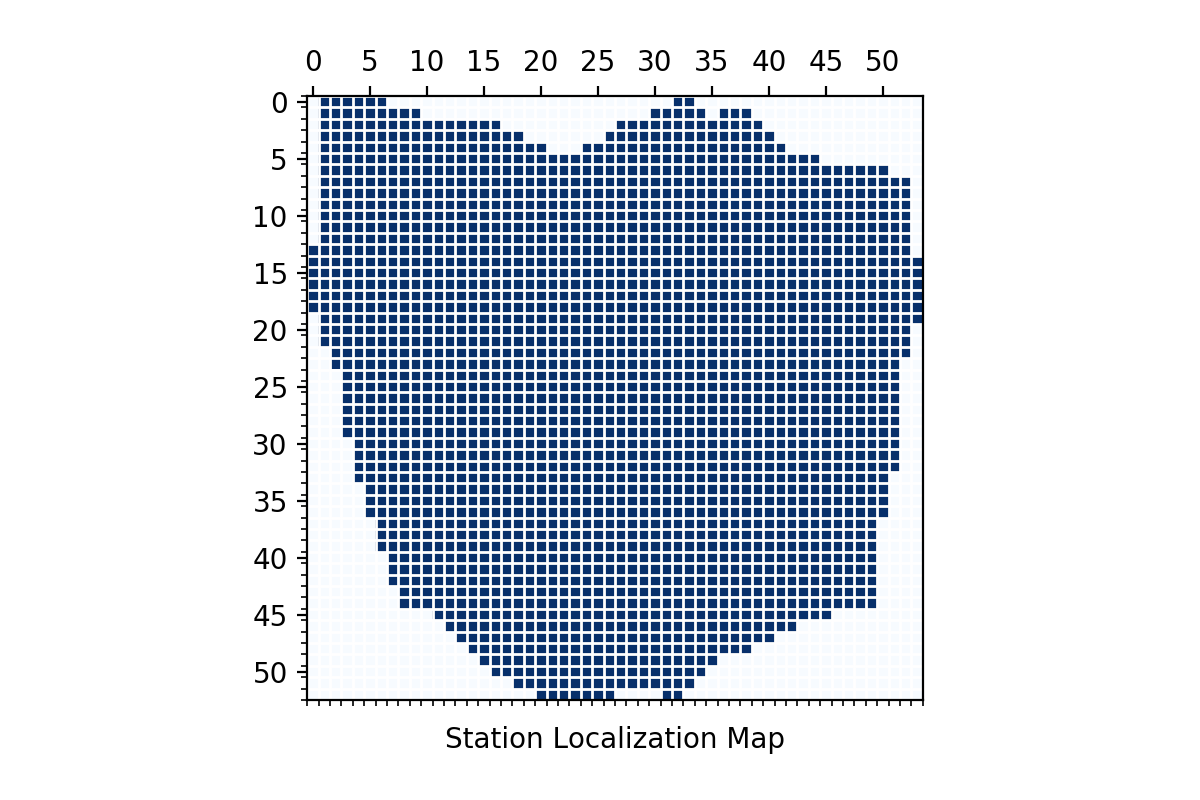
\includegraphics[width=0.8\textwidth]{station_location.png}
\caption{基站位置分布图}
\label{fig:2.1}
\end{figure}
图中显示,基站所覆盖区域被基站划分为54行53列的网格,对应2862个基站,且基站编号从网格左上角开始从左到右从上到下依次加一。图中红色网格代表提供人口流动数据的基站,蓝色网格则是无人区域。\\
\indent 基于此处理基站与网格分布关系,得到三个表格待后续分析使用:
\begin{itemize}
	\item基站编号---网格行列转换表
	\item 网格---基站编号转换表
	\item 无人区基站编号表
\end{itemize}
\subsubsection*{数据结构化、添补数据缺失}
数据范围是2017年9到11月人口流动数据。每天分24小时记录数据,每一行给出某天第几个小时第几号网格的,驻留人数、出发及到达人数。
为了便于后续数据处理,将数据形式进行处理。以驻留人数为例,每行表示某天某小时的所有基站数据,共2862列。无人区补零。
还有很少数的基站在一些时间点有数据缺失的情况,用该时刻前或后一时刻的数据填补。
\subsection{预处理和分析}
\subsubsection*{人流变化的短周期性}
观察以(15,30)为中心25个网格的一周内人口数量变化(见图\ref{fig:2.2}):
\begin{figure}[ht]
\centering
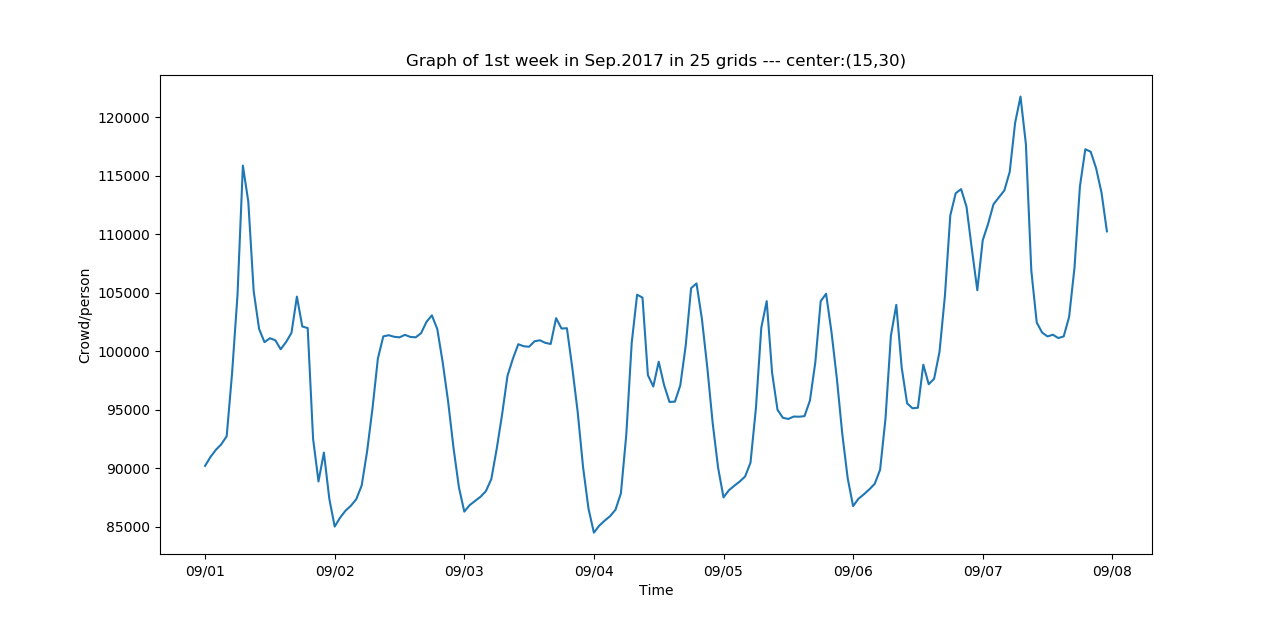
\includegraphics[width=0.8\textwidth]{month9_week1_25grids.png}
\caption{25个网格内人流一周内变化}
\label{fig:2.2}
\end{figure}
之所以取25个网格观察,是希望弱化网格间人口流量的影响,主要观察时序变化规律。
\indent 可以发现:
\begin{enumerate}
	\item 每天的人口驻留数量有明显的周期性变化。凌晨左右的人口数量最低。
	\item 已知09/02和09/03是周末,发现周末的人口数据与周中人口数据有所不同。
\end{enumerate}
\subsubsection*{人流变化的长周期性}
观察以(15,30)为中心25个网格的三周内人口数量变化,图(\ref{fig:2.3})中红线代表每周周六,可以看到人口数量在各周间也有所波动。
\begin{figure}[ht]
\centering
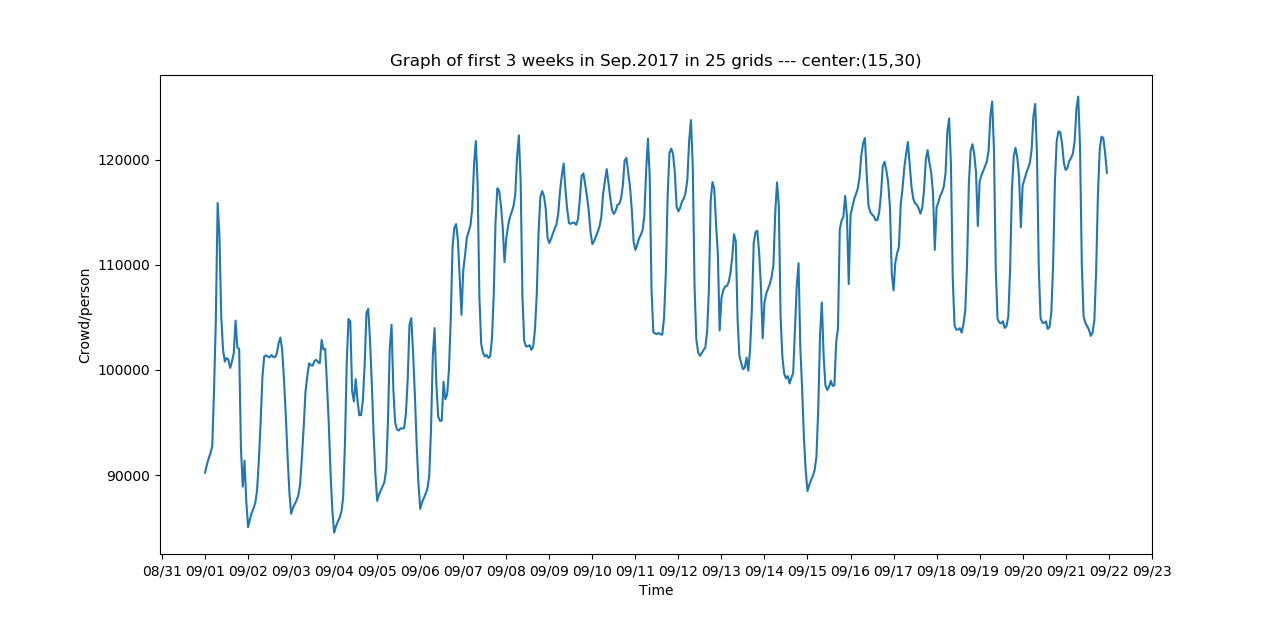
\includegraphics[width=0.8\textwidth]{month9_week3_25grids.png}
\caption{25个网格内人流三周内变化}
\label{fig:2.3}
\end{figure}
\subsubsection*{相邻地域的关联性}
以(15,30)(15,31)两个网格一天的人口流动为例,可以观测网格位置关联的地域的人流相关性。
\begin{figure}[ht]
\centering
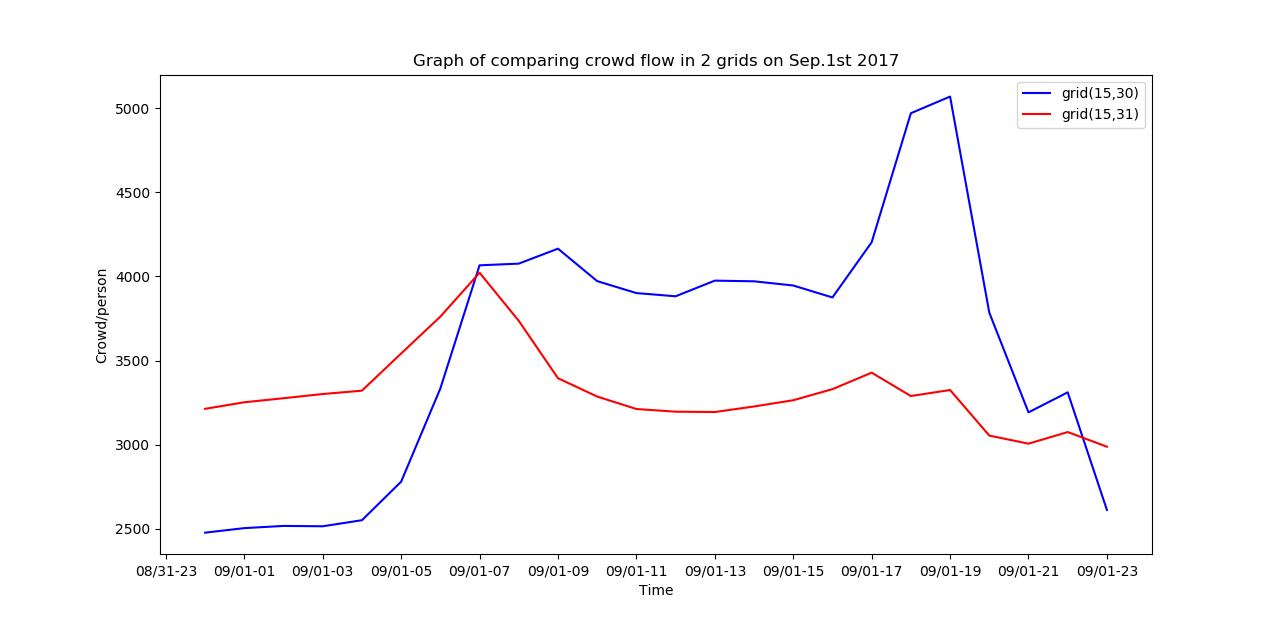
\includegraphics[width=0.8\textwidth]{compare.png}
\caption{两个相邻网格一天的人口流动}
\label{fig:2.4}
\end{figure}
\indent 从图(\ref{fig:2.4})中,
观察绿色框,可以发现一个网格人口增多另一个网格人口减少,其原因可能与人们在这两地移动相关,这在一定程度上体现网格位置对人口流动的影响。
\section{技术方案选择}
\subsection{可选技术方案}
\subsubsection*{ARIMA时序数据预测方法}
对于非平稳的时序序列,常常可以采用差分自回归移动平均模型(Autoregressive–moving-average model,ARIMA)进行分析\cite{whittle1966prediction,Hannan1970Multiple}。
在ARIMA(p,d,q)模型中,p 代表自回归阶数,d 代表差分次数, q 代表移动平均阶数,这一模型的建立需要解决以下三个问题:
\begin{enumerate}
	\item 利用差分将非平稳序列转化为平稳序列
	\item 通过模式识别确定模型属于AR、MA、ARMA中的哪一种
	\item 通过模式识别确定模型属于AR、MA、ARMA中的哪一种
\end{enumerate}
\indent 基于此,一种简单的预测方式可以对每个网格的时序序列进行建模求解,得到初步的预测情况。但是,网格的数量有两千两百多个,求解的计算量是较大的。同时,这样一来便没有考虑网格的位置分布关系对人口流动的影响。\\
\indent 基于这一模型的特点,比较适用于对于一些感兴趣的网络进行初步近似求解。
\subsubsection*{Res-CNN方法}
有文献\cite{Zhang2016Deep}指出,对于试图预测的某一时刻人口数量,在时序上,受到3个部分的影响:
\begin{itemize}
	\item $X_c$邻近时刻(例如之前的几个小时)
	\item $X_p$周期(例如昨天、前天的同一时刻)
	\item $X_q$趋势(例如上周、上上周等的同一时刻)
\end{itemize}
所以可以利用相同的网络结构来处理以上三部分信息。
\indent 另外,由于卷积层CNN通过卷积核的扫描融入了网格分布的位置信息,多个卷积层的叠加又可以使特征层次有小到大,所以文章先利用CNN对信息进行处理。
为了改善卷积层过深梯度消失的问题,在卷积层后加入了残差网络Res\ref{fig:2.5},从而构成了时序部分的网络结构。
\begin{figure}[ht]
\centering
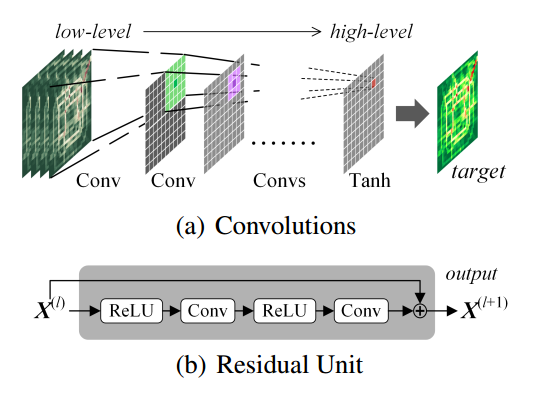
\includegraphics[width=0.8\textwidth]{Residual.png}
\caption{卷积层和残差单元}
\label{fig:2.5}
\end{figure}
最后,三个相同结构网络得到的数据,通过与参数矩阵相乘再相加的方式进行融合与维度的统一。同时训练得到了矩阵中的参数。
\\
\indent 另外,还可以考虑外部因素$E_t$(如天气等)对于人口流动的影响,其最终的网络结构如图(\ref{fig:2.6})所示。
\begin{figure}[ht]
\centering
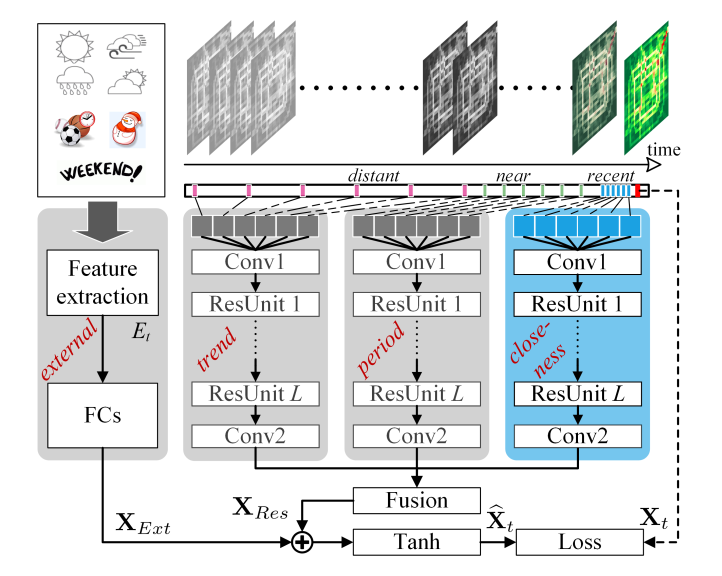
\includegraphics[width=0.8\textwidth]{net.png}
\caption{网络结构}
\label{fig:2.6}
\end{figure}
其中左侧是处理外部因素的,右侧是3个相似的卷积残差网络用来处理时序数据。将$E_t$转变成对应的特征向量,在其后连接两个全连接层FC。第一个全连接层可以看作对特征的提取,第二层则是为了获得与时序数据处理结果有相同维度。两部分最后的融合方式直接相加,并通过双曲正切函数控制在(-1,1)之间。网络的损失函数为预测与实际值误差的平方:
\begin{equation}
Loss = \Arrowvert y_t - \hat{y_t} \Arrowvert^2
\end{equation}
 
% Chapter 3

\chapter{技术路线及预测结果} 
\label{Chapter3}  
\section{技术路线选取}
基于之前的调研,在实际的预测分析中采取了三种方案进行预测分析:
\begin{itemize}
	\item 基于时间序列分析的Arima分析方法
	\item 多层感知机方法
	\item 时空残差网络方法
\end{itemize}
\section{Arima分析方法}
\subsection{模型概述}
如前文中所提到\ref{arima}, ARIMA模型全称为自回归积分滑动平均模型,主要用于时间序列预测。其主要思想为,将序列转化为平稳序列后,因变量的值由其滞后值与随机误差的现值和滞后值表示\cite{10.1007/978-981-10-8636-6_34}。其数学表达式如下:
\begin{equation}
\left( 1 - \sum _ { i = 1 } ^ { p } \phi _ { i } L ^ { i } \right) ( 1 - L ) ^ { d } X _ { t } = \left( 1 + \sum _ { i = 1 } ^ { q } \theta _ { i } L ^ { i } \right) \varepsilon _ { t }
\end{equation}
其中,$L$ 为滞后算子,$\phi$ 和 $\theta$ 为待求系数,$p$ 为自回归系数, $q$ 为滑动平均阶数,$d$为差分阶数
\subsection{分析过程}
以数据中第 \textbf{840} 号基站网格为中心的9个网格的每小时驻留人数的时序序列进行为例进行分析
\subsubsection*{检测序列是否平稳}
取两周的数据,观察序列的滑动平均与滑动方差(窗口长度为12),可以看到均值在较大范围内变化。进一步对序列差分,均值在很小范围内波动,基本可以视为平稳序列。
\begin{figure}[ht]
\centering
\subfloat[序列滑动平均]{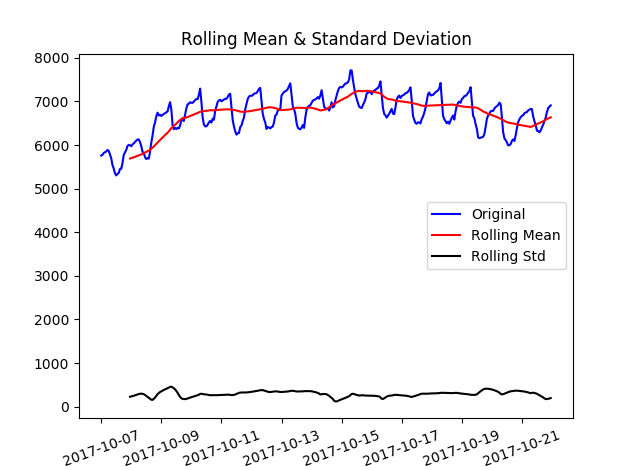
\includegraphics[width=0.50\textwidth]{ARIMA1.png}}
\subfloat[序列滑动方差]{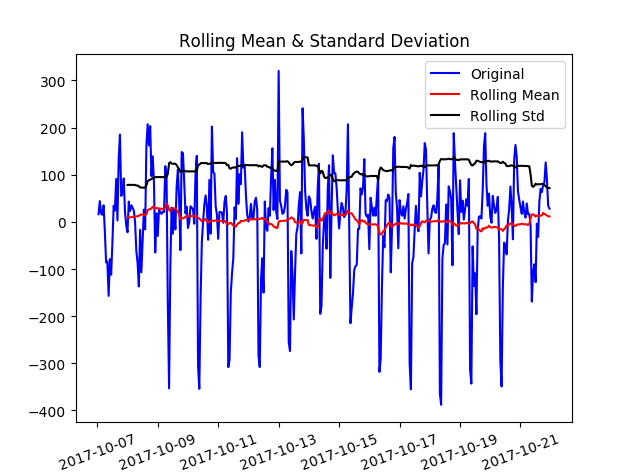
\includegraphics[width=0.50\textwidth]{ARIMA2.png}}
\hfill
\caption{检查序列是否平稳}
\label{fig:ARIMA1}
\end{figure}

\subsubsection*{对序列进行周期性和趋势性分解}
从图(\ref{fig:ARIMA3})中可以看出,数据有长期的变化趋势和明显的周期性变动,并且其残差项接近白噪声。

\begin{figure}[ht]
\centering
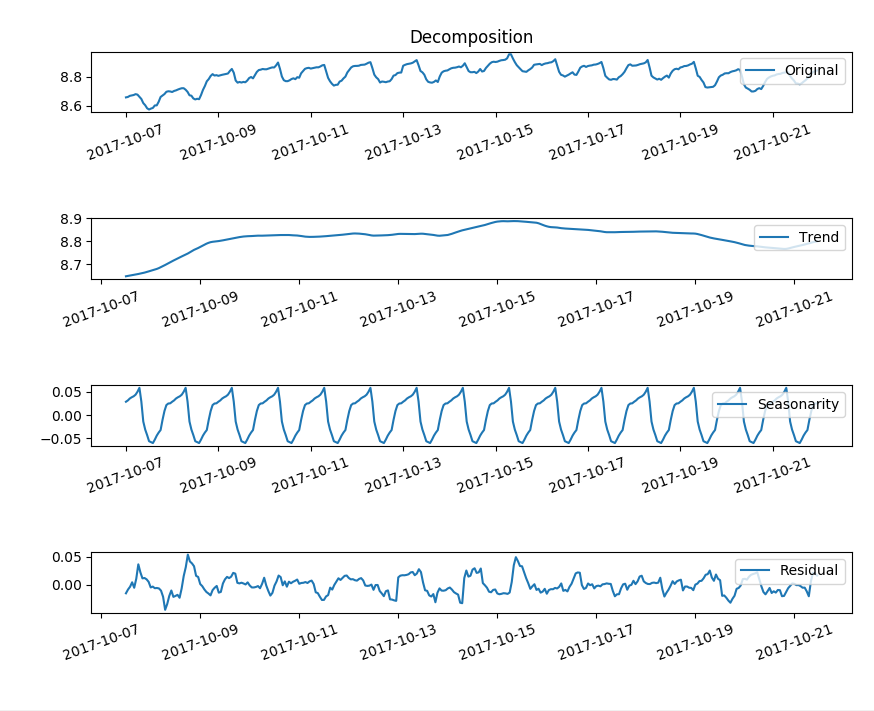
\includegraphics[width=0.8\textwidth]{ARIMA3.png}
\caption{序列周期性和趋势性分解}
\label{fig:ARIMA3}
\end{figure}

\subsubsection*{通过自相关和偏相关函数确定模型阶数}
从图(\ref{fig:ARIMA4})中可以观测出,依据自相关函数第一次降低到误差线以下可以确定MA阶数q=4,偏相关函数第一次降低到误差线以下可以确定AR阶数p=2。

\begin{figure}[ht]
\centering
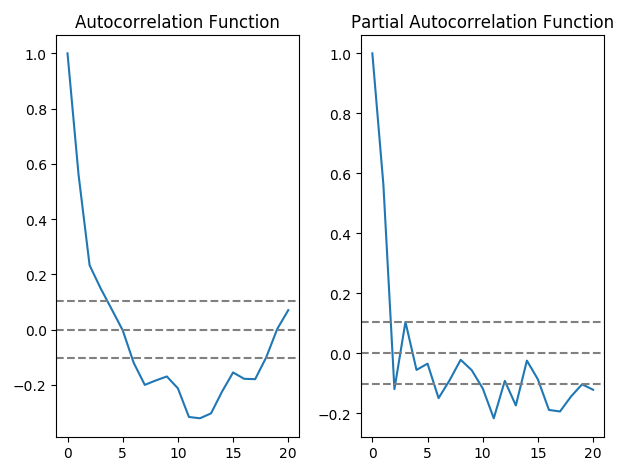
\includegraphics[width=0.8\textwidth]{ARIMA4.png}
\caption{确定模型阶数}
\label{fig:ARIMA4}
\end{figure}
\subsection{预测结果和分析}
最终的预测结果如图(\ref{fig:ARIMA5})所示,可以看出与原始序列对比,预测结果趋势一定程度与真值相近,但是峰值上存在较大误差。
\begin{figure}[ht]
\centering
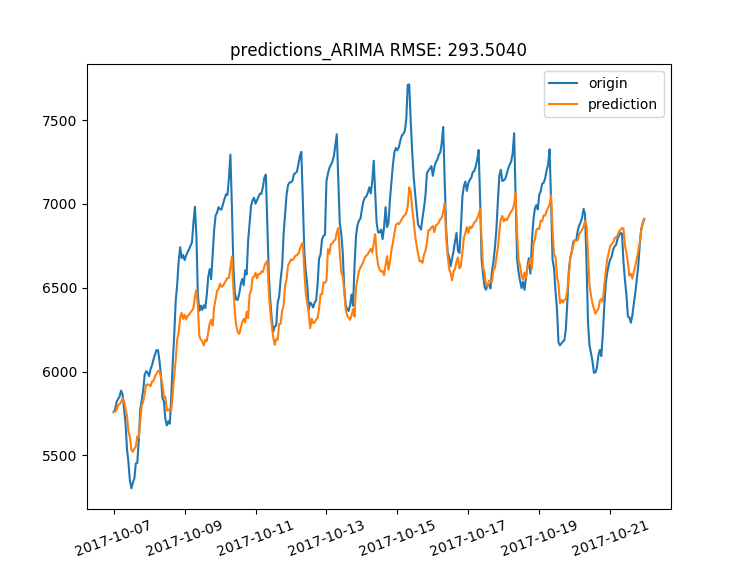
\includegraphics[width=0.8\textwidth]{ARIMA5.png}
\caption{预测结果}
\label{fig:ARIMA5}
\end{figure}
可以认为
\begin{enumerate}
	\item 利用Arima模型对本项目的数据进行建模可以预测趋势但是存在一定误差
	\item 可能的原因是序列的相关性是跳跃的,即某时刻的数据可能与1小时前、2两小时前、24小时前、48小时前、一周前的数据等相关性更高,而不是与之前的数据随时间间隔增大相关性逐渐降低
	\item 另外Arima模型所能考虑的空间上的范围也是有限的,其必然会导致预测精度上的误差
	\item 对于之后的模型建立,就需要考量时间相关性的构成和选取乃至对于空间上短程和长程相互影响的处理方法
\end{enumerate}


\section{时空残差网络方法}
\subsection{理论基础}
对于信令数据可以采取一下两种向量化方法:
\begin{equation}
\begin{split}
p = & f(id,time,week[weather,air condition,...])\\
p = & f(id,time,week,p(last hour),p(yesterday),p(last week),p(last month))
\end{split}
\end{equation}
其中,p 代表人口数据,可以通过维度的不同进行不同的表达(一维表示驻留人数,三维表示驻留人数,出发人数和到达人数),特别的,id 中隐含了地域的信息。
\subsection{分析手段}
采用有监督人工神经网络,期望输出为驻留人数、出发人数、到达人数,其基本架构如图(\ref{fig:3.1})所示。
\begin{figure}[ht]
\centering
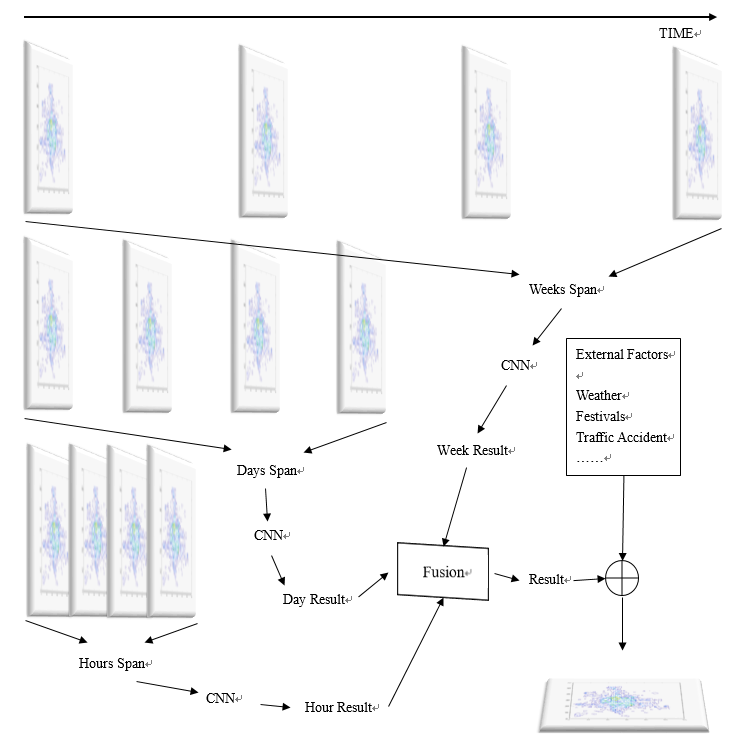
\includegraphics[width=0.8\textwidth]{ournet.png}
\caption{网络搭建基本构型}
\label{fig:3.1}
\end{figure}
输入为数据的特征,人工选取:我们认为主要以人数与 星期几(已有)、具体小时(已有)、位置(已有)、天气(可以爬取)、前一小时的人数(对已有数据处理)等主要因素有关。
同时我们以获得数据中的驻留人数、出发人数、到达人数作为标签,期望输出。
利用期望输出与网络输出之间的误差建立学习信号反向传播,修正网络权重。
\subsubsection*{初步网络搭建}
中间两个隐层,每个隐层20个神经元,采取全连接。
虽然说基站数量为2265个,我们的网络权重大约是600个待定参数好像不太够保存所有基站的信息。但是,注意到我们关注的是一片区域的总人口数据,而不是特指
某个基站的总人口个数,所以我们的网络只要区分出这种大概有同一人口特性的区域即可,最终对人口驻留,流动的分析也是基于区域进行分析的,所以600个左右的待定参数是够用的。
\subsubsection*{两种可能方案}
\begin{itemize}
	\item 方案A:多输入多输出(针对所有点的神经网络模型)\\
	类似于图片处理,2265个基站,输入即为2265*n,其中n为输入特征(星期,小时,ID(位置特征)等),输出为2265*3,3为标签个数(驻留人数、出发人数、到达人数)
	\item 方案B:少输入少输出(针对某一点的神经网络模型)\\
	针对某一个基站或者某一块区域进行训练。输入为特征个数(星期,小时,ID等),输出为3,即驻留人数、出发人数、到达人数。\\
	训练出来的模型是针对某一个基站或者某一块区域(9个基站左右,表示$9km^2$的一个区域)的人口情况。做分析时候要训练多点得到一个区域的数据进行分析。\\
	统计关心区域的总人口驻留,总人口流出,总人口流入来表示这个区域的人口数据。因为守恒关系,一个区域内所有点的人口驻留人数代数和即为该区域的总人口驻留人数,总人口流入与总人口流之差,即为该区域的总人口流入或总人口流出。
\end{itemize}


\subsection{方案设计}
最终的模型基于上述的 ARIMA 的初步分析和多层感知机的结果分析,参考文献中的方法,最终独立搭建了时空残差网络的模型方法。
\subsubsection*{问题建立}
对于人口数据,直观的显示是如图(\ref{fig:map})中显示的按照地图进行划分,而在我们的模型研究中,将其划分为沿着经纬线划分的$M \times N$矩形网格(见图\ref{fig:cluster})
\begin{figure}[ht]
\centering
\subfloat[基于地理信息地图的人流]{\label{fig:map}{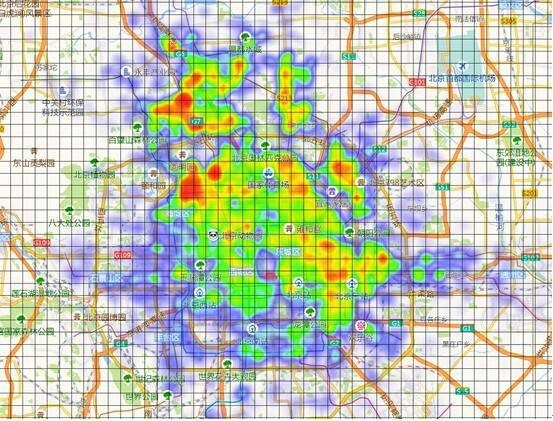
\includegraphics[width=0.45\textwidth]{map.jpg}}}
\subfloat[人流热力矩阵]{\label{fig:cluster}{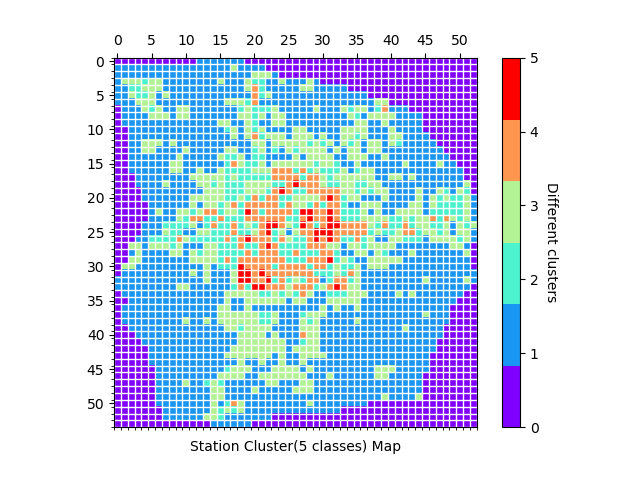
\includegraphics[width=0.45\textwidth]{clusters.png}}}
\hfill
\caption{北京人口区域划分:地理信息地图和人流热力图}
%\label{fig:subfigures}
\end{figure}
\subsubsection*{模型划分}
此问题实际上是想要基于过去的给定观测值进行未来的值的预测的一个回归分析的问题,其数学表达式为:
\\
给定 $\{X_t | t = 0,\cdots,n-1 \}$,预测 $X_{n},\cdots,X_{n+m}$
\subsubsection*{模型理论基础}
模型采用的深度残差网络相比传统的卷积神经网络可以有着更深的结构层数\cite{he2016deep},而实践证明其在图像分类、物体识别等问题中有着相当好的应用效果\cite{he2016identity},所以我们基于这样的网络结构进行模型的搭建。\\
一般地,在残差网络中可以将回归预测模型的问题定义为:
\begin{equation}
X^{(l+1)} = X^{(l)} + \mathcal{F}(X^{(l)})
\end{equation}
其中,$X^{(l+1)}$和$X^{(l)}$分别是第$l$个残差单元的输入和输出,而$\mathcal{F}$为残差函数,而实际上网络的目标就是基于输入值寻找到合适的残差函数,一个典型的残差单元的示意如图(\ref{fig:resident})所示。
\begin{figure}[ht]
\centering
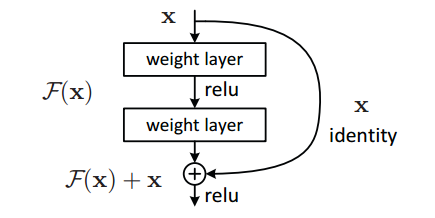
\includegraphics[width=0.8\textwidth]{resident.png}
\caption{残差单元示意图\cite{he2016deep}}
\label{fig:resident}
\end{figure}
\subsubsection*{残差网络结构}
前文的图(\ref{fig:3.1})很好地展示了本研究所采用的残差网络的架构,在时间周期层面上考虑 \textbf{小时、天、周}三个不同层次的影响,并利用卷积考虑空间上的相互关联,最后再加入外部因素的影响。 模型分别采取预测时刻的最近三个小时、一天前的四个小时和一周前的两个小时的数据作为输入,在网络中得到不同的权重,再计算残差实现反向传播。\\
\indent 在实际的网络设计中,考虑到城市不同区域之间的相互关联(如依靠地面公路、地铁的流动)进行卷积核的大小的调整和对于激活函数的定义。
\subsubsection*{数据混合}
模型中的三个不同时间周期的数据可以用参数矩阵的方法进行混合:
\begin{equation}
\mathbf { X } _ { R e s } = \mathbf { W } _ { hour } \circ \mathbf { X } _ { hour }  + \mathbf { W } _ {day } \circ \mathbf { X } _ { day }  + \mathbf { W } _ { week } \circ \mathbf { X } _ { week } 
\end{equation}
其中的乘法为矩阵乘法(哈达马积),而参数$W_{hour}$,$W_{day}$和$W_{week}$为模型参数
\subsubsection*{模型算法和优化方法}
模型的算法步骤和优化方法见算法框图(\ref{al}) 
\begin{algorithm}[t]
\caption{ResNet Training Algorithm} %算法的名字
We first construct the training
instances from the original sequence data.\\ Then, RenNet is trained via backprogagation and Adadelta.\\
\hspace*{0.02in} {\bf Input:} %算法的输入, \hspace*{0.02in}用来控制位置,同时利用 \\ 进行换行
Historical observations: \{ $X_0,\cdots,X_{n-1}$ \}\\
\hspace*{0.02in} Lengths of closeness, period, trend sequences: $l_c$,$l_p$,$l_q$\\
\hspace*{0.02in} Period, trend span: q\\
\hspace*{0.02in} {\bf Output:} %算法的结果输出
learnt ResNet model\\
\begin{algorithmic}[1]
\State \#construct training instances\\
D <- None % \State 后写一般语句
\For{t in all available time interval [1,n-1]} % For 语句,需要和EndFor对应
  \State $S_c = [X_{t-l_c},X_{t-(l_c-1)},\cdots,X_{t-1}]$
	\State $S_p = [X_{t-l_p*p},X_{t-(l_p-1)*p},\cdots,X_{t-p}]$
	\State $S_q = [X_{t-l_q*q},X_{t-(l_q-1)*q},\cdots,X_{t-q}]$\\
Put an training instance ($\{S_c,S_p,S_q \},X_t$) into D
\EndFor
\# define the loss
\\
LOSS = MSE($X_t$,output of ResNet)\\
\# train the model\\
\# initialize all learnable parameters cita in ResNet\\
Epoch <- int(numbers)

\For{epoch in range(Epoch)} % For 语句,需要和EndFor对应
  \State \textbf{Repeat}
	\State Select an instance $D_b$ from D
	\State $\theta$ by minimizing the LOSS with $D_b$
\textbf{Until} all elements of D used\\
\# save model every 10 epoches
  \If{epoch \% 10 == 0} % If 语句,需要和EndIf对应
    \State Save model
  \EndIf
\EndFor
\end{algorithmic}
\label{al}
\end{algorithm}
% Chapter 4

\chapter{分析和结论} % Main chapter title

\label{Chapter4} 
\section{数据分析}
\subsection{数据集和预处理}
测试数据集(见表\ref{table:data})是由中国联通智慧足迹数据科技有限公司所提供的从2017.9.1.-2017.11.30.的北京六环内的手机信令结果。 数据实验中选取从 2017.9.7.-2017.11.23.的数据为训练集,而之后的一周即2017.11.24-2017.11.30.的数据为测试集。
\begin{table}
\centering
\caption{数据集}
\label{table:data}
\begin{tabular}{p{0.3\columnwidth}|p{0.45\columnwidth}}
\hline
\hline
\textbf{Dataset} & \textbf{PopuBJ}\\
\hline
Data Type& Iphone Signal\\
\hline
Location & Beijing\\
\hline
Time Span & 9/1/2017-11/30/2017\\
\hline
Time interval & 1 hour\\
\hline
Grid map size & (53,54)\\
\hline
\hline
\end{tabular}
\end{table}
\subsection{模型比较}
将模型的预测结果和下面两种基线结果进行比较:
\begin{itemize}
	\item 插值方法(naive model):用历史平均来插值预测,对于某一ID,某一周,某一时刻,计算它的历史平均
	\item 多层感知机模型(MLP),即常规的深度神经网络
\end{itemize}
\subsection{评估方法}
采取均方残差(RSME)的方法进行预测结果的精度分析,其数学表达式\cite{friedman2001elements}为:
\begin{equation}
R M S E = \sqrt { \frac { 1 } { z } \sum _ { i } \left( x _ { i } - \hat { x } _ { i } \right) ^ { 2 } }
\end{equation}
其中,$\hat{x_i}$和$x_i$分别是预测值和真实值,而$z$代表所有的数据的个数。
\section{预测结果}
\begin{table}
\centering
\caption{不同预测方法均方残差比较}
\label{table:RSME}
\begin{tabular}{p{0.3\columnwidth}|p{0.45\columnwidth}}
\hline
\hline
\textbf{Model} & \textbf{RMSE}\\
\hline
Deep-ST& Iphone Signal\\
\hline
Location & Beijing\\
\hline
Time Span & 9/1/2017-11/30/2017\\
\hline
\hline


\end{tabular}
\end{table}

% Table generated by Excel2LaTeX from sheet 'demandData'
\subsection{不同模型和不同参数下的预测结果}
表(\ref{tab:diffpara})中的模型1到模型4对应的参数和优化方法分别为:
\begin{itemize}
	\item模型1\\ 初始学习率为0.1,学习衰减指数0.95,优化方法AdadeltaOptimizer
	\item模型2 \\初始学习率0.01,学习衰减指数1, 优化方法GradientDescentOptimizer (该优化方法在本模型很容易不收敛)
	\item模型3\\ 初始学习率0.01, 学习衰减指数0.999,优化方法AdadeltaOptimizer
	\item 模型4 \\初始学习率0.001, 学习衰减指数0.999999999,优化方法AdadeltaOptimizer
\end{itemize}
以其中的模型1为例进行说明,可以看出在从一天到七天的预测周期内,其预测的准确率都要高于插值预测模型,而不同参数之间的预测准确率也会发生改变,另外根据图(\ref{fig:acc})中可以更加清楚的看出,不同模型的预测精度均随着预测时间点的后移而下降。\\
总结而言,建议在实际的预测分析中应该逐天分析,因为随着天数的增加,误差会越来越大并逐渐累积(这是一个显自然的结果),所以从整个星期来衡量而言预测精度会受到影响。另外,逐天分析可以
知道预测出的结果在一定的误差范围下可接受的预测天数是多少天。比方说前三天预测比插值得来的结果好很多,到第四天开始精度和插值一样,后面插值会比模型的精度大等情况在实际的预测中都是有可能发生的。
\begin{table}[htbp]
  \centering
  \caption{不同参数组合对于预测精度的影响}
    \begin{tabular}{rrrrrrrrr}
    \hline
           &       &       &       &\multicolumn{1}{l}{error<50} &       &       &       &  \\\\
           \hline
          & \multicolumn{1}{l}{24h} & \multicolumn{1}{l}{48h} & \multicolumn{1}{l}{72h} & \multicolumn{1}{l}{96h} & \multicolumn{1}{l}{120h} & \multicolumn{1}{l}{144h} & \multicolumn{1}{l}{168h} &  \\
          \hline
    \multicolumn{1}{l}{模型1} & 45.66\% & 42.49\% & 41.17\% & 40.52\%  & 40.07\% & 39.83\% & 39.82\% &  \\
    \multicolumn{1}{l}{模型2} & 53.01\% & 46.02\% & 42.34\% & 39.96\% & 38.22\% & 36.76\% & 35.60\% &  \\
    \multicolumn{1}{l}{模型3} & 48.80\% & 43.20\% & 40.19\% & 38.37\% & 37.10\% & 36.10\% & 35.35\% &  \\
    \multicolumn{1}{l}{模型4} & 51.49\% & 43.94\% & 39.96\% & 37.40\% & 35.46\% & 33.91\% & 32.70\% &  \\
    \multicolumn{1}{l}{插值} & 40.07\% & 40.59\% & 40.80\% & 40.68\% & 40.46\% & 40.27\% & 40.16\% &  \\
    \hline
          &       &       &       &       &       &       &       &  \\
          &       &       &       &\multicolumn{1}{l}{error<100} &       &       &       &  \\ \\
          \hline
          & \multicolumn{1}{l}{24h} & \multicolumn{1}{l}{48h} & \multicolumn{1}{l}{72h} & \multicolumn{1}{l}{96h} & \multicolumn{1}{l}{120h} & \multicolumn{1}{l}{144h} & \multicolumn{1}{l}{168h} &  \\
          \hline
    \multicolumn{1}{l}{模型1} & 61.11\% & 57.28\% & 55.52\% & 54.71\% & 54.18\% & 53.39\% & 53.39\% &  \\
    \multicolumn{1}{l}{模型2} & 71.79\% & 62.78\% & 57.56\% & 53.90\% & 51.10\% & 48.76\% & 46.84\% &  \\
    \multicolumn{1}{l}{模型3} & 67.35\% & 59.42\% & 55.17\% & 52.37\% & 50.29\% & 48.63\% & 47.36\% &  \\
    \multicolumn{1}{l}{模型4} & 69.63\% & 59.75\% & 54.03\% & 49.98\% & 46.84\% & 44.29\% & 42.23\% &  \\
    \multicolumn{1}{l}{插值} & 50.34\% & 51.40\% & 51.73\% & 51.56\% & 51.27\% & 50.99\% & 50.82\% &  \\
     \hline
          &       &       &       &       &       &       &       &  \\
          &       &       &       &\multicolumn{1}{l}{error<200} &       &       &       &  \\ \\
          \hline
          & \multicolumn{1}{l}{24h} & \multicolumn{1}{l}{48h} & \multicolumn{1}{l}{72h} & \multicolumn{1}{l}{96h} & \multicolumn{1}{l}{120h} & \multicolumn{1}{l}{144h} & \multicolumn{1}{l}{168h} &  \\
          \hline
    \multicolumn{1}{l}{模型1} & 77.11\% & 73.98\% & 72.43\% & 71.93\% & 71.46\% & 71.13\% & 71.12\% &  \\
    \multicolumn{1}{l}{模型2} & 88.73\% & 80.81\% & 75.62\% & 71.59\% & 68.24\% & 65.24\% & 62.53\% &  \\
    \multicolumn{1}{l}{模型3} & 85.45\% & 78.03\% & 73.86\% & 70.82\% & 68.38\% & 66.34\% & 64.63\% &  \\
    \multicolumn{1}{l}{模型4} & 87.59\% & 78.74\% & 72.47\% & 67.51\% & 63.37\% & 59.82\% & 56.70\% &  \\
    \multicolumn{1}{l}{插值} & 63.19\% & 64.52\% & 64.87\% & 64.59\% & 64.12\% & 63.74\% & 63.48\% &  \\
    \hline
    \end{tabular}%
  \label{tab:diffpara}%
\end{table}%

\begin{figure}[ht]
\centering
\subfloat[绝对误差小于50的格点占比]{\label{fig:acc}{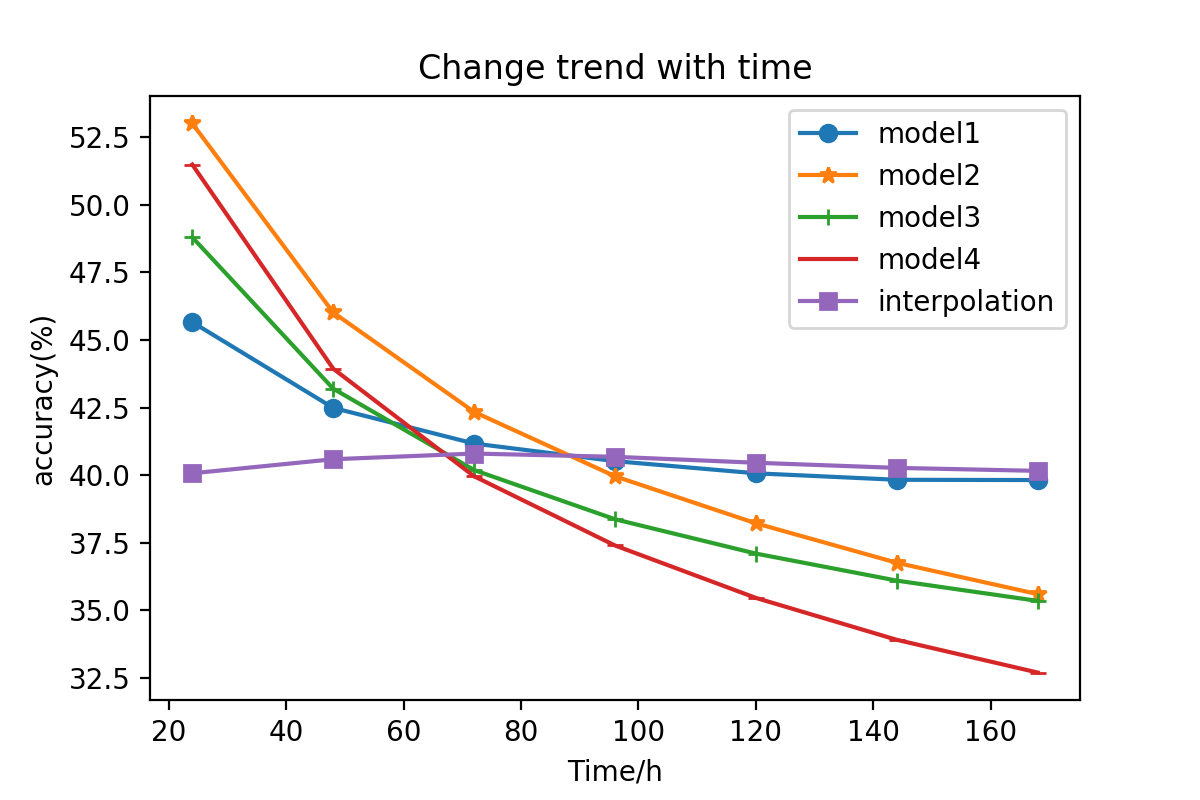
\includegraphics[width=0.45\textwidth]{accuracy.png}}}
\subfloat[均方误差变化]{\label{fig:rsmeacc}{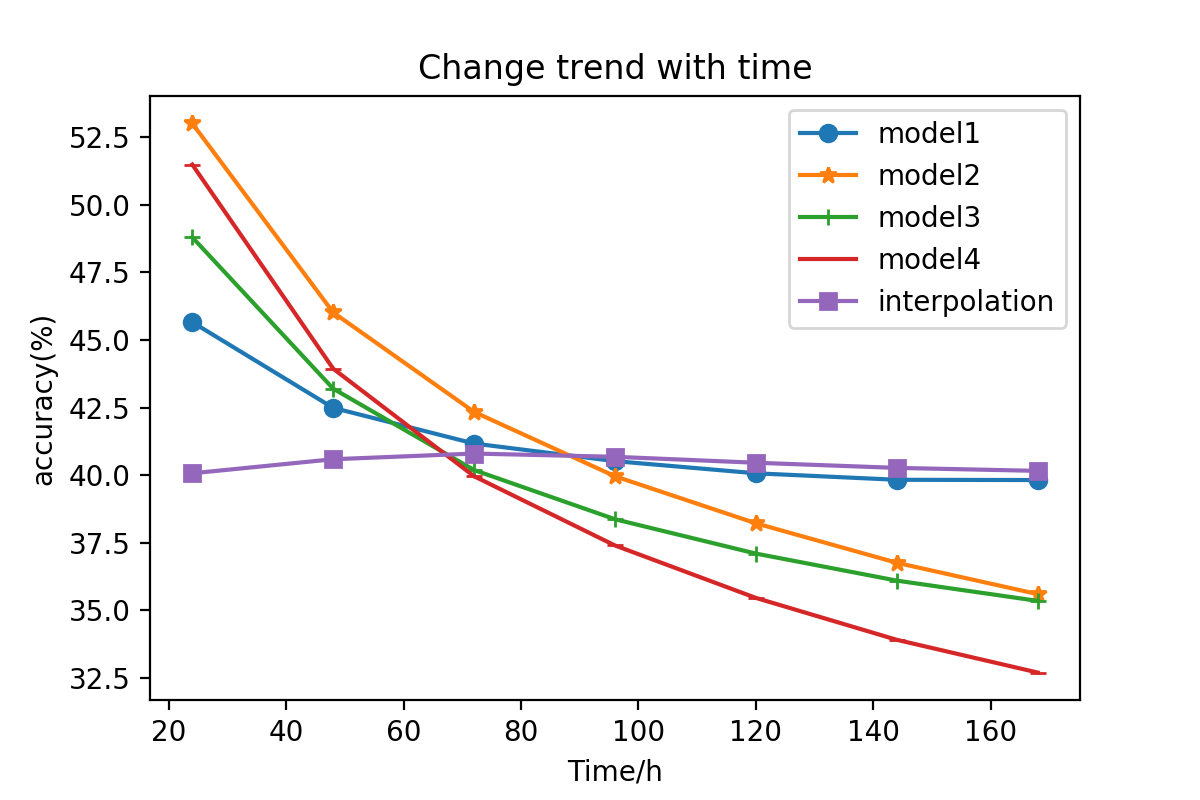
\includegraphics[width=0.45\textwidth]{accuracy.png}}}
\hfill
\caption{模型预测精度随着预测时间的变化}
%\label{fig:subfigures}
\end{figure}
加上RSME的误差分析部分
\subsection*{参数的影响}
上面的分析表明,所设计的残差网络在预测的精度上无论是简单的深度神经网络还是和均值比较都有较大的提升,而从表(\ref{table:diffpara})中也可以看出,采用不同的参数对于残差网络训练结果的影响:
\begin{itemize}
	\item 初始学习率
	\item 学习衰减指数
	\item 优化方法
\end{itemize}
\subsection{结果可视化和区域分析}
对于预测结果可以分别采用热力图和结合地理信息的人流地图加以可视化,如图(\ref{fig:peopleheatmap})所示:

\begin{figure}[ht]
\centering
\subfloat[人口热力图]{\label{fig:heatmap}{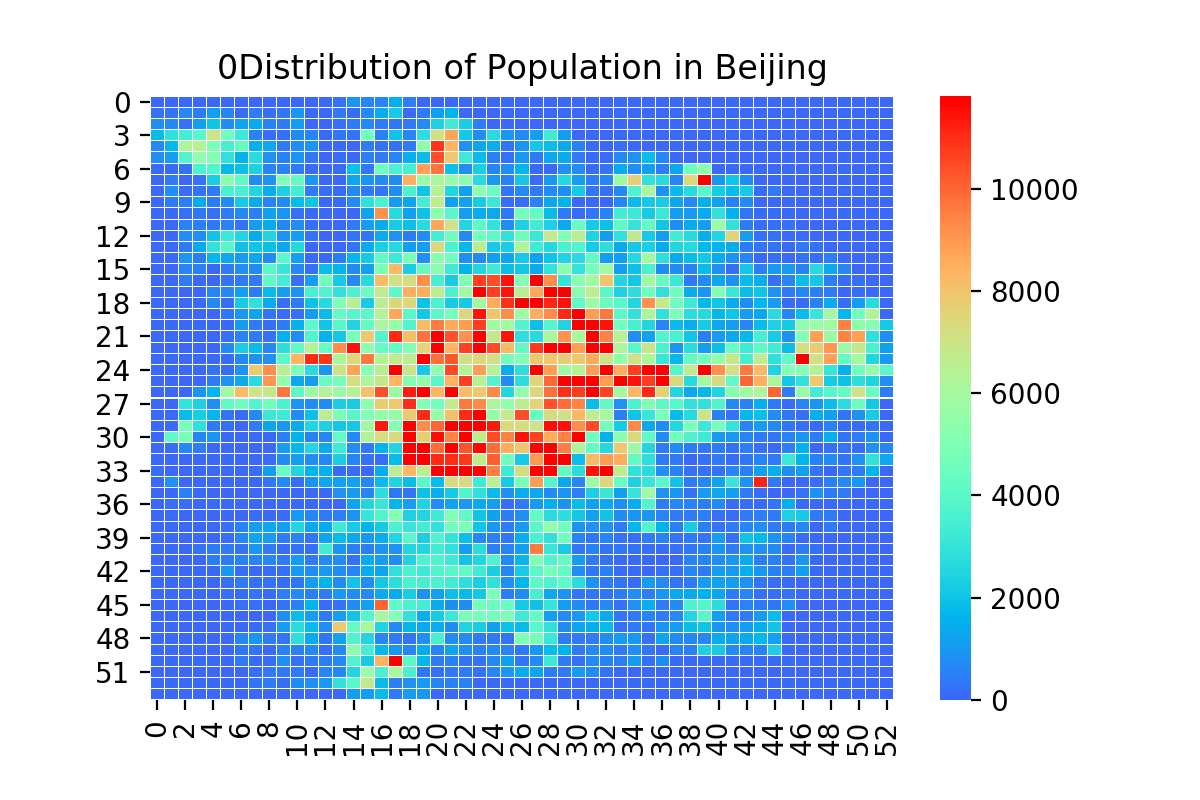
\includegraphics[width=0.45\textwidth]{heatmap.png}}}
\subfloat[结合实际地理信息的可视化]{\label{fig:folium}{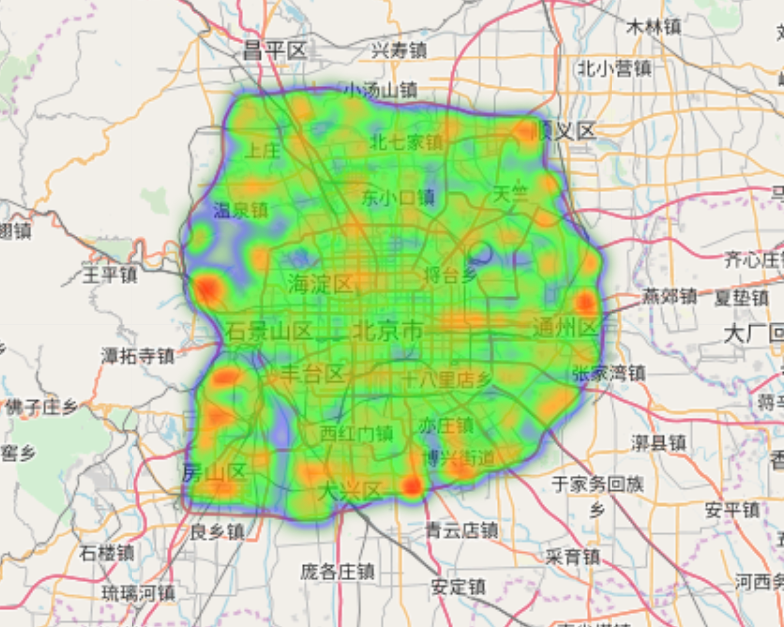
\includegraphics[width=0.45\textwidth]{folium.png}}}
\hfill
\caption{人口分布预测结果可视化}
\label{fig:peopleheatmap}
\end{figure}
而更进一步的,在对于全局预测效果的评估的基础上,可以更加细致的对于具体的特征地区进行预测结果的分析:
\begin{figure}[ht]
\centering
\subfloat[三里屯]{\label{fig:11}{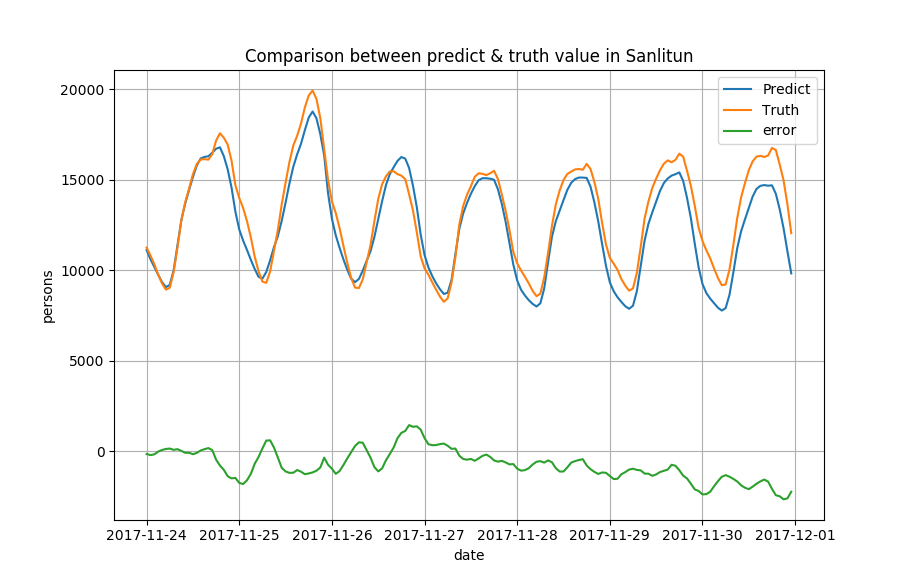
\includegraphics[width=0.45\textwidth]{region1.png}}}
\subfloat[天安门]{\label{fig:22}{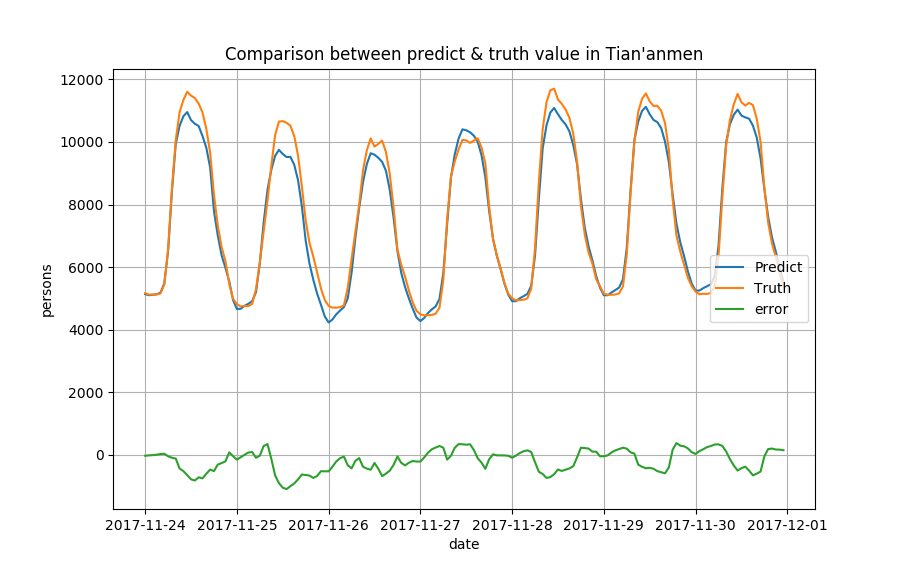
\includegraphics[width=0.45\textwidth]{region2.png}}}
\hfill
\subfloat[北京西站]{\label{fig:33}{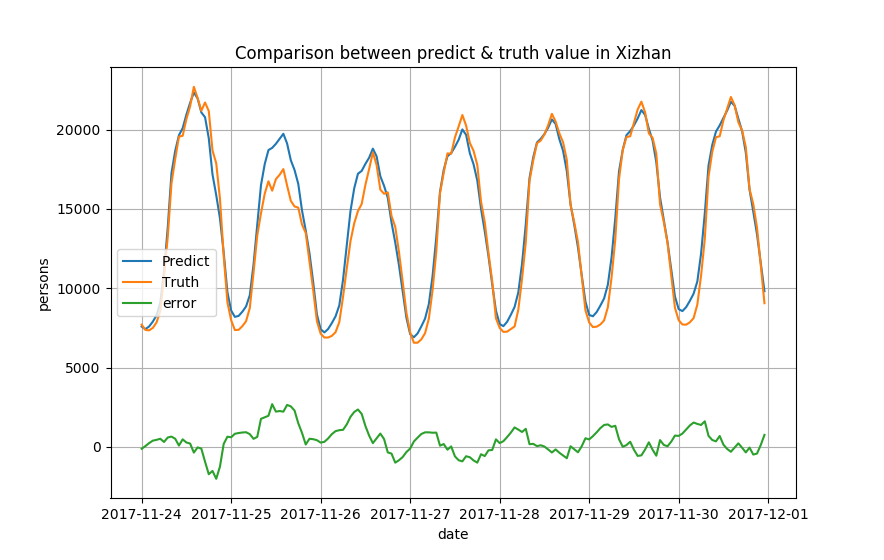
\includegraphics[width=0.45\textwidth]{region3.png}}}
\subfloat[中关村]{\label{fig:44}{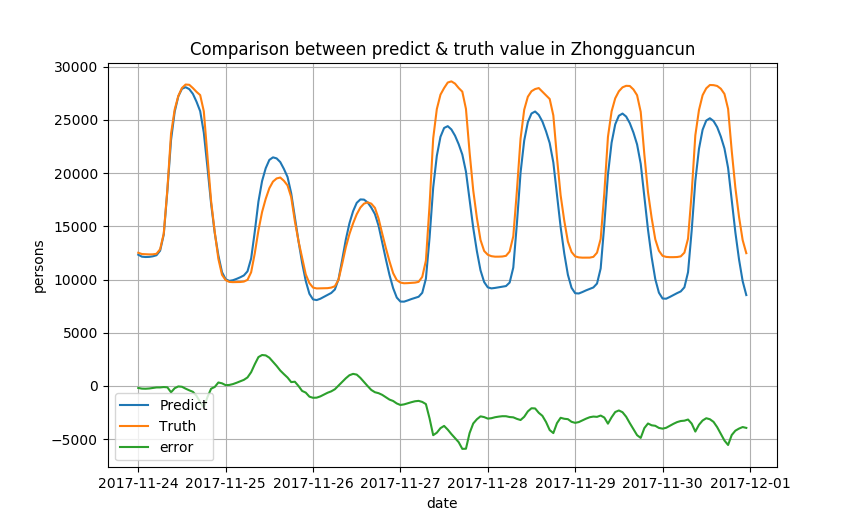
\includegraphics[width=0.45\textwidth]{region4.png}}}
\caption{四个典型地区的预测结果和真实值比较}
\label{fig:region}
\end{figure}
图(\ref{fig:11})展示了三里屯地区的人流量预测情况及其与真实值之间的对比关系,从曲线的走势可以看出,总体上预测值和真实值的符合度比较高,误差值在前期的分布没有明显的趋势性,表明造成预测误差的一个重要原因可能是随机因素的影响,而预测的后期也呈现出一定的预测精度的下降趋势,这也和之前的讨论分析是相符合的。\\
而图(\ref{fig:33})中展示了北京西站这样一个人流量较大但也有较明显变化的区域的预测结果,可以看出,对于高峰的预测是相对比较准确的,可以看出本模型可以在诸如火车站、地铁站等的人流预测和预警中发挥较好的作用。

\section{总结和展望} 
%\include{Chapters/Chapter5} 

%----------------------------------------------------------------------------------------
%	THESIS CONTENT - APPENDICES
%----------------------------------------------------------------------------------------

\appendix % Cue to tell LaTeX that the following "chapters" are Appendices

% Include the appendices of the thesis as separate files from the Appendices folder
% Uncomment the lines as you write the Appendices

% Appendix A

\chapter{技术说明文档} % Main appendix title
\label{AppendixA} % For referencing this appendix elsewhere, use \ref{AppendixA}
\section{数据细节说明}
数据总量:大约60万条数据,大小200M
\begin{enumerate}
	\item 将三个月的数据合并,并且加上新属性(星期),后续会加上天气
	数据列名:
	DATE(date:2017-09-01)	TIME(INT)		WEEK(INT)	ID(INT)	NUMS(INT)	GONUMS(INT)	REANUMS(INT)
	\item 找到不同ID基站之间的地理位置关系。即将ID与地图对应
	\item 对异常数据的讨论 \\
	找出了数据有缺失的ID,分别为:\\
	\begin{table}
	\label{tb:id}
	\centering
	\caption{数据有缺失的ID}
	\begin{tabular}{c|c}
	\hline
	\hline
	ID & 1913(1162) \\
	ID & 1860(1209) \\
	ID & 1914(1417) \\
	ID & 1754(1443) \\
	ID & 1915(1593) \\
	ID & 1806(1790) \\
	ID & 1866(2060) \\
	ID & 1966(2149) \\
	ID & 2017(2178) \\
	ID & 1863(2183) \\
	\hline
	\hline
	\end{tabular}
	\end{table}
	括号内为基站出现的次数,满次为2184
	\item 处理基本思路:
	\begin{itemize}
		\item 舍弃
		\item 补全
	\end{itemize}
		a.舍弃
		b.补全
	\item 准备完成将数据转换为tensorflow数据集文件tfrecords工作,包括预处理
\end{enumerate}
\section{项目进度控制}
项目的进度分为以下几个阶段:
\begin{enumerate}
  \item 第一阶段:11.07之前\\
  完成以下工作:
  \begin{itemize}
    \item 问题背景调研:包括问题的背景、对应的客户的需求、和应用的市场前景,形成对需求分析、产品调研、应用案例的阶段性报告
    \item 对于问题结果可视化的研究:预期结果的产出形式
    \item 对于数据的清洗和初步分析
    \begin{itemize}
      \item 数据清洗: 将数据格式化为和具体网格相关联的数据并进行重新划分和编号以进行进一步的计算
      \item 初步分析:对于数据进行诸如聚类,对于时空分布规律进行简单探究和分析,基于对于其周期性规律的认识乃至天气等因素的影响的认识建立模型的建构
    \end{itemize}
    \item 技术实现的方案选择和可行性调研
    \begin{itemize}
      \item 利用现有文献中的数据集和代码,实际测试其方法可行性,总结技术要点和技术难点
      \item 对于文献中提及的其他方法,如ARIMA、SARIMA、VAR、DeepST方法进行调研,针对其在这一问题上的应用可行性和所存在的问题进行总结分析
      \item 基于以上两点,进行技术路线的设计以及对于可行性和预期结果的分析。
    \end{itemize}
  \end{itemize}
  \item 第二阶段:11.07-11.28\\
  完成整个系统的搭建和模型验证,得出预测的结果和预测的精度
  \item 第三阶段:11.29-12.05\\
  进行系统的优化和特征深入分析,如对于算法中对于各种影响因素和处理手段的体现和对于结果的影响\\
  \item 第四阶段:12.06-12.15\\
  对工作进行总结和分析
\end{enumerate}
工作的基本逻辑架构如图(\ref{fig:A1})所示:
\begin{figure}[ht]
\centering
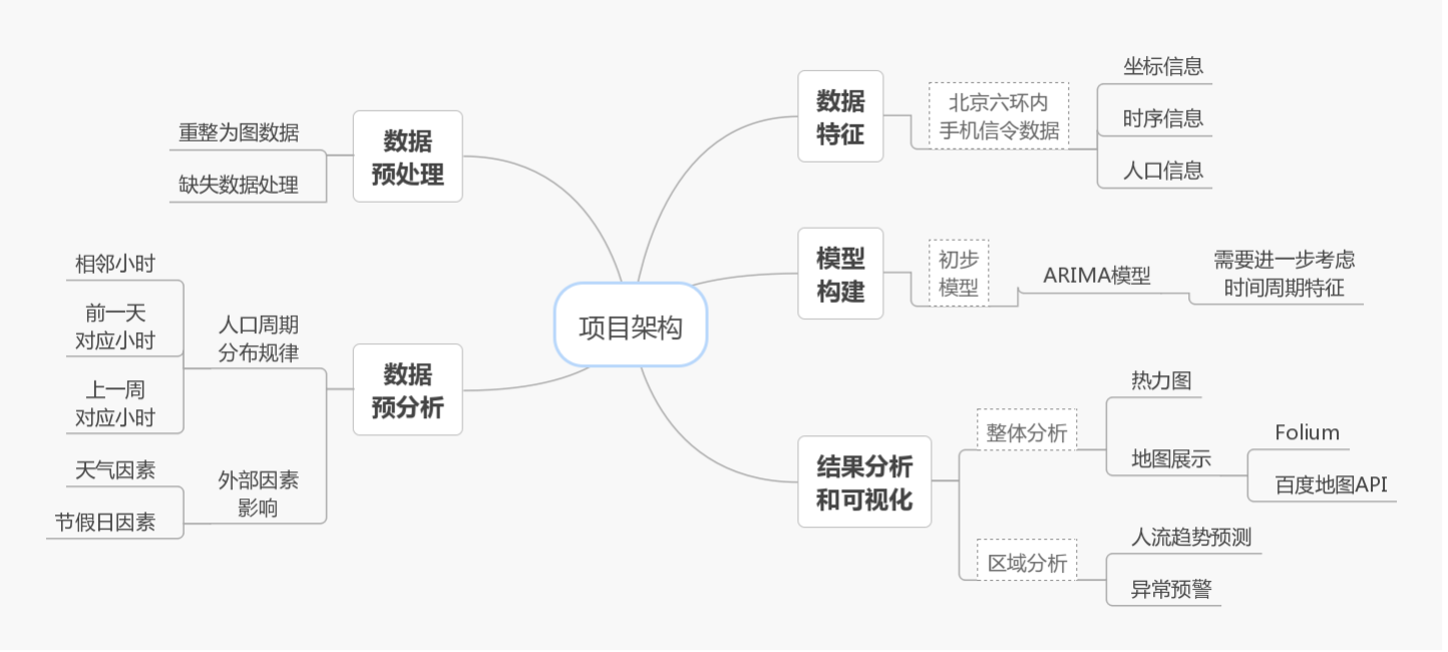
\includegraphics[width=\textwidth]{timeline.png}
\caption{网络搭建基本构型}
\label{fig:A1}
\end{figure}
% Appendix B

\chapter{系统构建} % Main appendix title
\label{AppendixB} % For referencing this appendix elsewhere, use \ref{AppendixA}
\section{模型功能和系统实现}

本项目代码和文档开源于Project-Unicom \\ \url{https://github.com/BigDataSystemTHU2018/Project-Unicom}

\subsection{系统架构}
如图(\ref{fig:pattern})所示,整体模型架构分为数据预处理和预分析,模型构建,结果可视化和后分析三个层次。
\begin{figure}[ht]
\centering
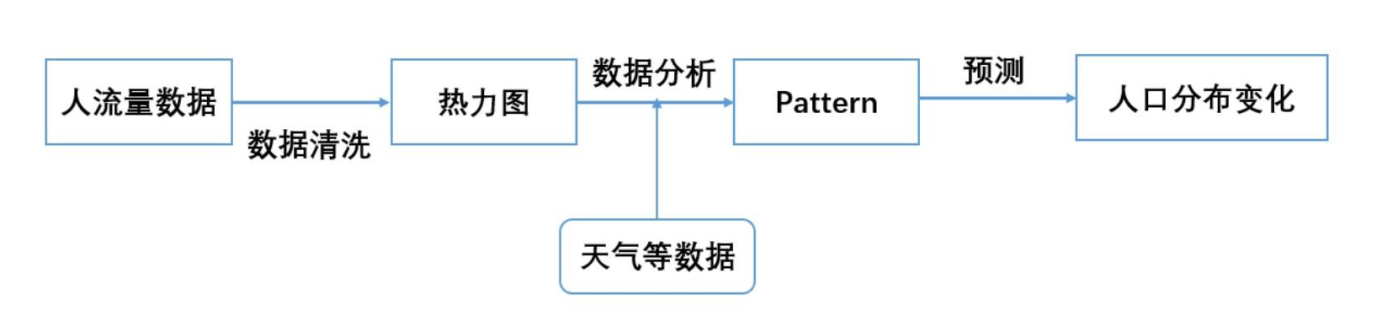
\includegraphics[width=0.8\textwidth]{pattern.png}
\caption{项目分析思路}
\label{fig:pattern}
\end{figure}
\subsection{代码架构}
分析代码见 \\ \url{https://github.com/BigDataSystemTHU2018/Project-Unicom/tree/master/Code}
问题的主要模块分析如下:
\begin{itemize}
	\item 问题分析阶段
		\begin{itemize}
			\item 问题描述:用过去三个月的信令数据预测未来一个周的人口分布,即已知过去三个月的数据,(尽可能)预测未来一周的数据
			\item 问题性质:回归
			\item 评判指标:预测出的结果尽可能的准确,即预测值与实际误差尽可能小。
		\end{itemize}
	\item 设计阶段——设计出一个回归系统,输入为过去三个月的数据,输出为已有数据的分析结果和预测结果。系统包含以下几个模块:
		\begin{itemize}
			\item 预处理模块:
			输入为原始数据,输出为清洗后的数据。负责数据的清洗,缺失值补全,异常值噪声点的处理等
			\item 预分析模块:
			负责从已有数据中提取挖掘先验知识,数据初步分析,可视化等。
			\item 回归前处理模块:
			将数据归一化等。
			\item 回归器模块:
			用于预测
			\item 回归后处理模块:
			包括可视化,对预测数据分析,生成报告等等。
		\end{itemize}
	\item 编码阶段——技术路线:
		\begin{itemize}
			\item 平台:tensorflow,sklearn
			\item 算法:聚类(K-means),降维(PCA/NMF),回归(MLP/ResNet)
			\item 可视化:matlab, matplotlib(seaborn)
		\end{itemize}
\end{itemize}
\subsubsection*{回归器结构}
回归系统的回归器分为4个部分,分别是:数据处理、Resnet搭建、网络训练、模型预测,其代码见\\ \url{https://github.com/BigDataSystemTHU2018/Project-Unicom/tree/master/Code/Processor/ResNet})\\ 模块的主要功能为:
\begin{enumerate}
	\item 从本地目录获取所有清洗好的数据,将数据按照Resnet的要求加载到内存。
	\item 对数据自动分为训练数据和预测数据,其中训练数据喂入Resnet进行模型训练。
	\item 对训练好的模型进行预测结果的输出。
	\item 支持断点续训,训练过程中模型会每10轮保存一次,可以自由跳转到已经保存好的模型进行继续训练或者模型输出。
	\item 支持迁移学习。即利用已经训练好的模型训练新的场景,提高训练的效率和降低对样本数量的需求。
	\item getdataTHU.py: 搜索当前目录下所有.csv,.txt文件,以这些文件作为所需的数据。请将待训练的数据放入当前目录。
	\item ResnetTHU.py: 定义网路结构,可以根据需要改变卷积核大小(CONV\_SIZE)和激活函数。
	\item trainTHU.py: 训练模块,也为反向传播模块,根据需要可以改变图片大小
	IMAGE\_WIDTH,IMAGE\_HIGHT,改变通道数NUM\_CHANNELS1,\\
	NUM\_CHANNELS2,NUM\_CHANNELS3,同时BATCH\_SIZE2,BATCH\_SIZE3\\,BATCH\_SIZE4也要相应的改变来保持一致(现为取最近3小时,一天前的4小时,一周前的2小时)。
	\item predictTHU.py: 预测模块,需要设置预测天数(现为7天)。
\end{enumerate}
模型网络的基本逻辑架构如图(\ref{fig:B1})所示:
\begin{figure}[ht]
\centering
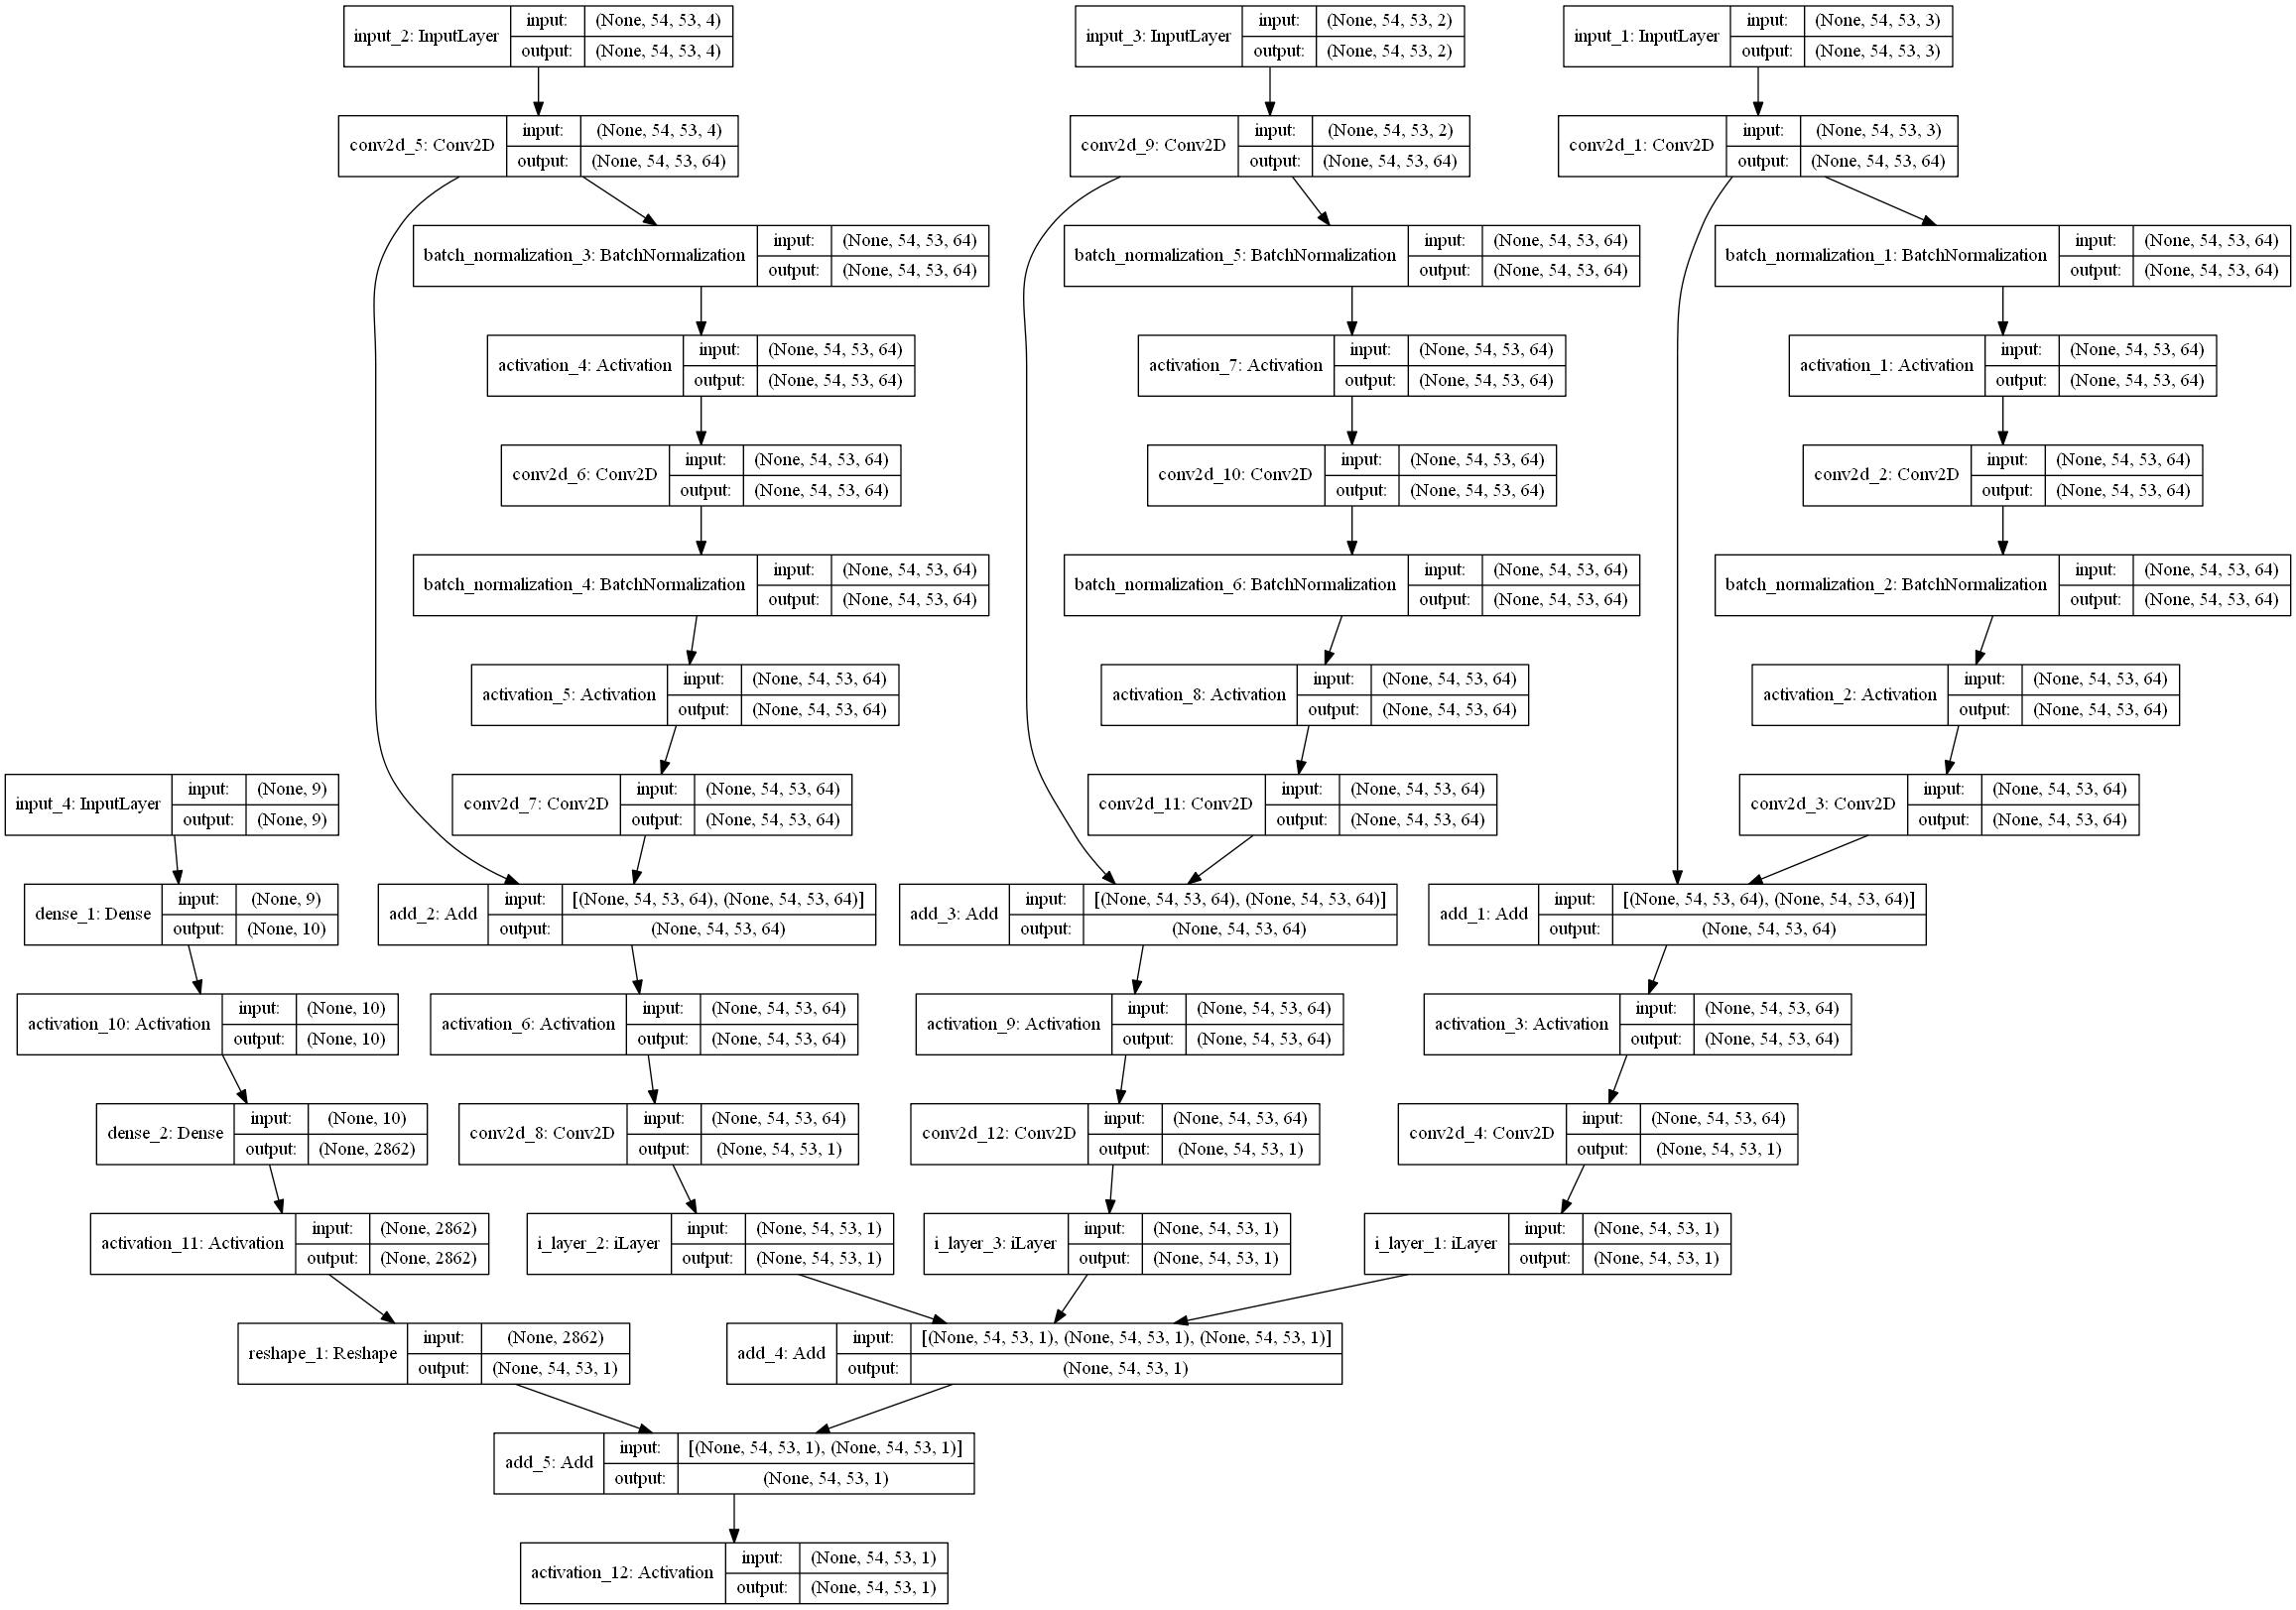
\includegraphics[width=0.8\textwidth]{B2.png}
\caption{残差网络构型}
\label{fig:B1}
\end{figure}

%\include{Appendices/AppendixC}

%----------------------------------------------------------------------------------------
%	BIBLIOGRAPHY
%----------------------------------------------------------------------------------------

%\printbibliography
\bibliographystyle{unsrt}
\bibliography{ref}
%----------------------------------------------------------------------------------------

\end{document}  
